\documentclass{template/openetcs_report}
% Use the option "nocc" if the document is not licensed under Creative Commons
%\documentclass[nocc]{template/openetcs_article}
\usepackage{lipsum,url}
\usepackage{supertabular}
\usepackage{multirow}
\usepackage{color, colortbl}
\usepackage{hyperref}
%\usepackage{listings}
\usepackage{makeidx}
\definecolor{gray}{rgb}{0.8,0.8,0.8}
\usepackage[modulo]{lineno}
\graphicspath{{./template/}{.}{./images/}}

\newcommand{\define}[1]{\index{#1}\emph{#1}}

\begin{document}
\frontmatter
\project{openETCS}

%Please do not change anything above this line
%============================

%user specified macros
%\newenvironment{activity}[2][planned]
	{\begin{tabular}{p{0.25\textwidth}@{\hspace{0.05\textwidth}}p{0.7\textwidth}}
			\multicolumn{2}{p{\textwidth}}{\colorbox{black}{\begin{minipage}{1.1cm}\begin{center}\textsc{\footnotesize \textcolor{white}{#1}}\end{center}\end{minipage}}~~\textbf{#2}}\\
	}
	{\end{tabular}}

\newcommand{\entry}[2]{#1:&#2\\}
\newcommand{\website}[1]{Website:&\url{#1}\\}
\newcommand{\desc}[1]{\multicolumn{2}{p{\textwidth}}{#1}\\}

\newcommand{\VV}{Verification \& Validation\xspace}
\newcommand{\vv}{verification \& validation\xspace}

\newcommand{\tbd}{\colorbox{cyan}{\%\%To Be Defined\%\%}}
\newcommand{\tbc}{\colorbox{cyan}{\%\%To Be Confirmed\%\%}}
\newcommand{\todo}[1]{\colorbox{cyan}{\%\%{#1}\%\%}}
\newcommand{\nthng}[1]{}

% The document metadata is defined below

%assign a report number here
\reportnum{OETCS/WP3/D3.5.1.2}

%define your workpackage here
\wp{Work-Package 3: ``Modeling''}

%set a title here
\title{openETCS System Architecture and Design Specification}

%set a subtitle here
\subtitle{Second Iteration: Scope of openETCS ITEA2 Functions}

%set the date of the report here
\date{October 2014}


%document approval
%define the name and affiliation of the people involved in the documents approbation here
\creatorname{Baseliyos Jacob}
\creatoraffil{DB Netz}

\techassessorname{[assessor name]}
\techassessoraffil{[affiliation]}

\qualityassessorname{Izaskun de la Torre}
\qualityassessoraffil{SQS}

\approvalname{Klaus-R\"udiger Hase}
\approvalaffil{DB Netz}


%define a list of authors and their affiliation here

\author{Baseliyos Jacob, Bernd Hekele}

\affiliation{DB Netz AG\\
  V\"olckerstrasse 5\\
  D-80959 M\"unchen Freimann, Germany}

\author{Marc Behrens}
\affiliation{DLR}

\author{David Mentre}
\affiliation{Mitsubishi Electric R\&D Centre Europe}

\author{Jos Holtzer, Jan Welvaarts, Vincent Nuhaan}
\affiliation{NS}

\author{Jacob G\"artner}
\affiliation{LEA Engineering}

% define the coverart
\coverart[width=350pt]{openETCS_EUPL}

%define the type of report
\reporttype{Architecture and Functional Specification}


\begin{abstract}
%define an abstract here
This document gives an introduction to the architecture of openETCS. The functional scope is tailored to cover the functionality required for the openETCS demonstration as a target of the ITEA2 project: the Utrecht Amsterdam use-case. It has to be read as an add-on to the models in SysML, Scade and to additional reading referenced from the document.
\end{abstract}

%=============================
\maketitle

%Modification history
%if you do not need a modification history table for your document simply comment out the eight lines below
%=============================


\chapter*{Modification History}
\tablefirsthead{
\hline 
\rowcolor{gray} 
Version & Section & Modification / Description & Author \\\hline}
\begin{supertabular}{| m{1.2cm} | m{1.5cm} | m{6.6cm} | m{3.7cm} |}
0.1 & Document & Initial document providing the structure & Baseliyos Jacob \\\hline
0.2 & Document & Workshop Results included and some pretty-printing & Bernd Hekele \\\hline

\end{supertabular}

% list subsubsections in table of contents
\setcounter{tocdepth}{3}


\tableofcontents
\listoffiguresandtables
\newpage
%=============================

%Uncomment the next line if you need line numbers for tracebility when the document is in review
%\linenumbers
%=============================


% The actual document starts below this line
%=============================

\mainmatter

\chapter{Introduction}

\section{Assumption and Preconditions}
\begin{itemize}
\item All future contributions shall be fully aligned an compliant with final documents
\item Alls documents produced by the partners with i.e. constrains with document; other contributions will be discarded
\end{itemize}

\section{Process}
\begin{itemize}
\item Alstom as WP 3 leader will be responsible for planning
\item Time and quality aspects
\item openETCS tools and methodology
\end{itemize}


\section{Functions ERTMS/ETCS}


The ERTMS / ETCS system was developed with a view to interoperability of trains on the 
different European rail networks. It is divided into "tracks" - and "board" finishes 
and shall establish a mutual message operation, by beacons or through a "radio" - 
The transmission system (in this case a mobile telephone network GSM-R) is performed. 
It defines several operating levels, and the system must also interfaces with the 
existing monitoring systems of the trains (using STM) have. 
The ERTMS / ETCS system provides the transport operator (the track) the choice of conditions 
concerning the use and operation. 
The train must therefore may go with different operating conditions on routes. 
Thus has the onboard equipment but must be implemented, 
to the interoperability of the train to ensure on the other networks. 
These functions must therefore correspond to one standard: the SRS (version 3.4.0). 

application functions, which have two different species of origin: 
defined in the SRS: here one finds in particular the 
speed monitoring- and transfer functions; these functions 
must be implemented in full accordance with the SRS; they can in 
indeed be on any network on which the train is used; these functions 
are described below in Section \ref{SRSFunction}; 


Moreover, there are functions to adapt to the train: so, for example, the processing 
a "separation distance" in the airborne equipment trigger: 
This is dependent on the distribution of functions between the 
Control monitoring equipment (which the ERTMS / ETCS), and the other 
CCS Systems.

\section{openETCS Architecture: Iterations and History}

The openETCS Architecture and Design is implemented in iterations \cite{deployment}. The current step (second iteration) is based on a step to implement the kernel functions of the ETCS system \cite{firstIteration}. For a better understanding of the scope the Iteration is described in the following.

\subsection{First Iteration Functional Scope: The Minimum OBU Kernel Function}
\label{sec:FunctionalScopeTheMinimumOBUKernelFunction}

The openETCS first iteration architecture and the design of the openETCS OBU software as mainly specified in \cite{subset-026} UNISIG Subset\_026 version\_3.3.0. 

The appropriate functionality has been divided into a list of functions of different complexity (see the WP3 function list \cite{functions}).

All these functions are object of the openETCS project and have to be analysed from their requirements and subsequently modelled and implemented. With limited manpower, a reasonable selection and order of these functions is required for the practical work that allows the distribution of the workload, more openETCS participants to join and leads to an executable---limited---kernel function as soon as possible. 

While the first version of this document focuses on the first version of the limited kernel function, it is intended to grow in parallel to the growing openETCS software.

The first objective of the first iteration was
\begin{itemize}
	\item ``Make the train run as soon as possible, with a very minimum functionality, and in the form of a rapid prototype.''
\end{itemize}
This does not contradict the openETCS goal to conform to EN50128.
\begin{itemize}
	\item After a phase of prototyping, the openETCS software shall be implemented in compliance to EN50128 for SIL4 systems.
\end{itemize}

\subsection{How to find the functions of the First Iteration in the Architecture}
The functions will be merged with the new architecture. Wherever a function has already been in the scope it will be marked as "first iteration".

\section{Glossary and Abbreviations}

\textbf{API} Application Programming Interface\\
\textbf{EVC} European Vital Computer\\
\textbf{BTM} Balise Transmission Module\\
\textbf{SRS} System Requirements Specification\\


\textbf{SRS-Subset 26}\\
\textbf{QA-Plan: D1.3.1}\\
\textbf{Process: D2.3}\\
\textbf{Methods: D2.4}\\
\textbf{API: D2.7}\\

\chapter{The openETCS Architecture}


\begin{figure}[hbtp]
\chapter{SRS Architecture}
\centering
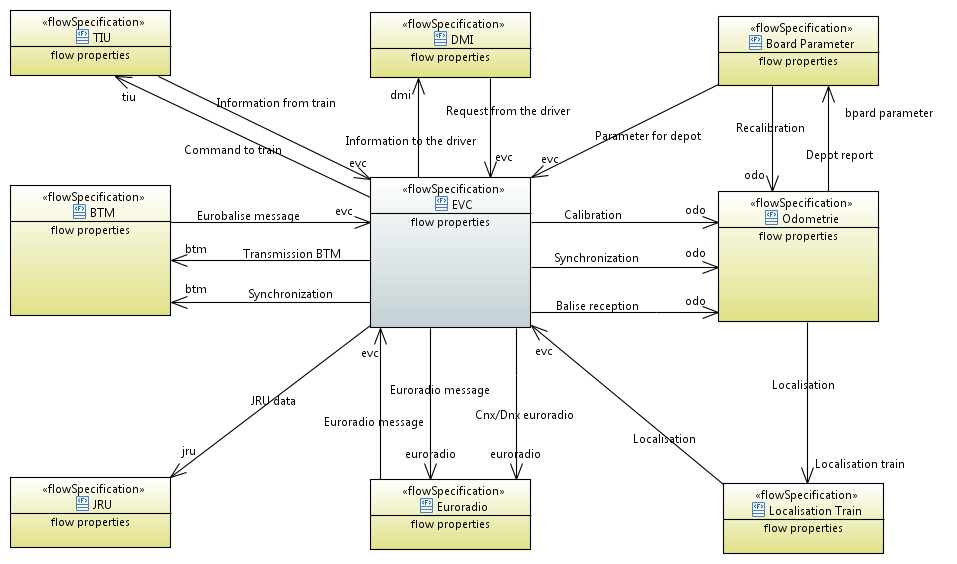
\includegraphics[angle=90, scale=0.9] {images/HighLevelArchitecture.png}
\caption{SRS architecture}
\end{figure}



\begin{figure}[hbtp]
\chapter{Functional Breakdown}
\centering
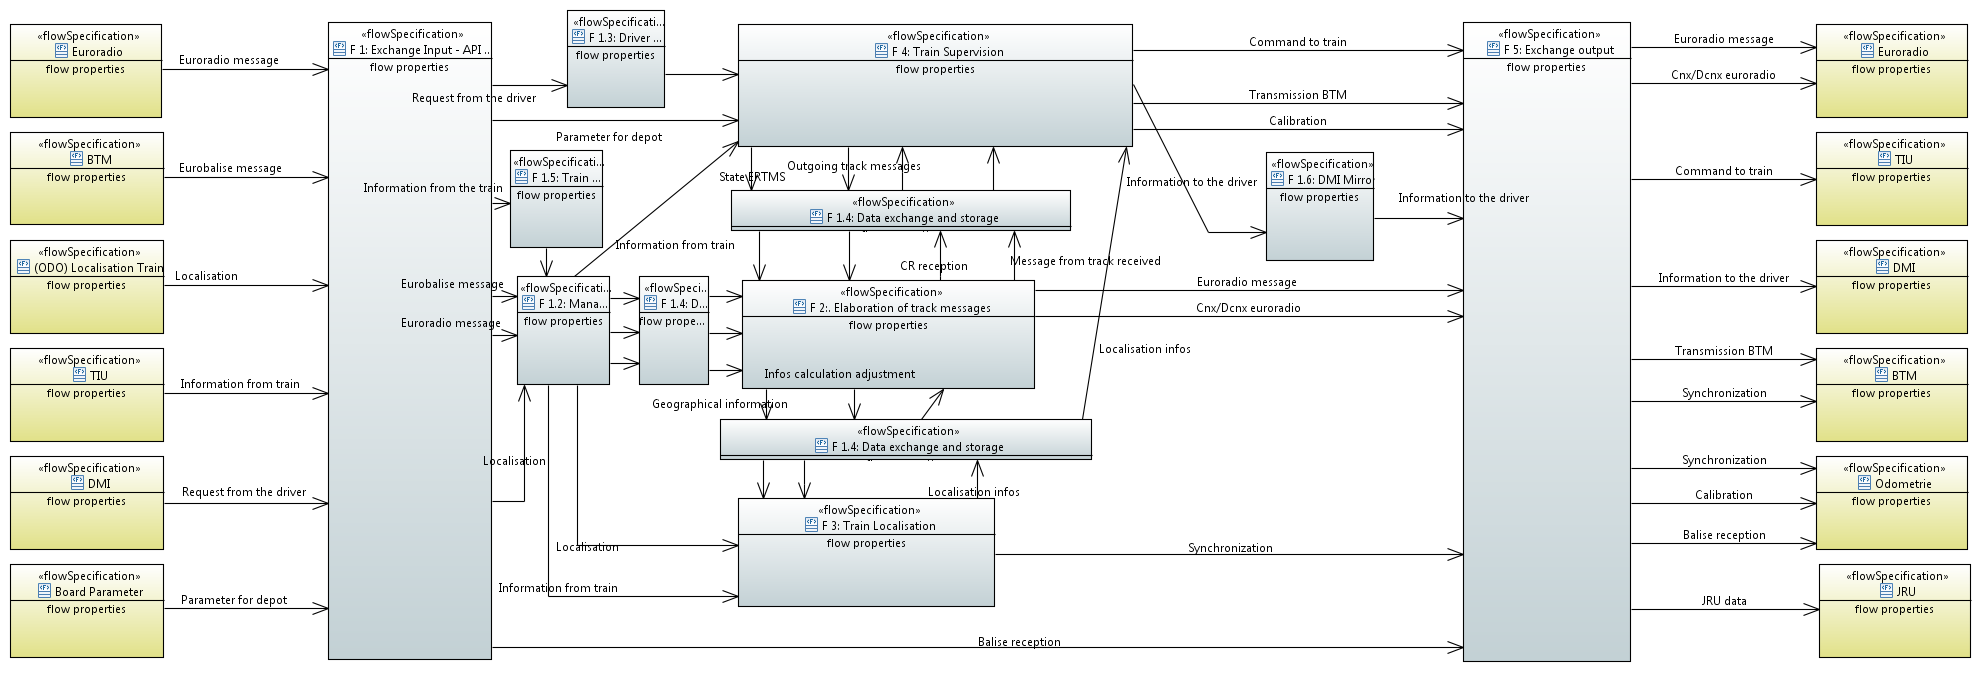
\includegraphics [angle=90, scale=0.45] {images/HighLevelFunctionalbreakdown}
\caption{SRS Breakdown}
\end{figure}
\newpage



\chapter{Description of the SRS Functions}
\label{SRSFunction}

\section{Reference abstract hardware architecture}

\subsection{Why a reference abstract hardware architecture?}

For proper understanding of openETCS API and of constraints imposed on
both sides of the API, we need to define a \define{reference abstract hardware architecture}. This hardware architecture is ``abstract''
is the sense that the actual vendor specific hardware architecture
might be totally different of the abstract architecture described in
this chapter. For example, several units might be grouped together on
the same processor.

However the actual vendor specific architecture shall fulfil all the
requirements and constraints of this reference abstract hardware
architecture and shall not request additional constraints.

\subsection{Definition of the reference abstract hardware architecture}

\begin{figure}
  \centering
  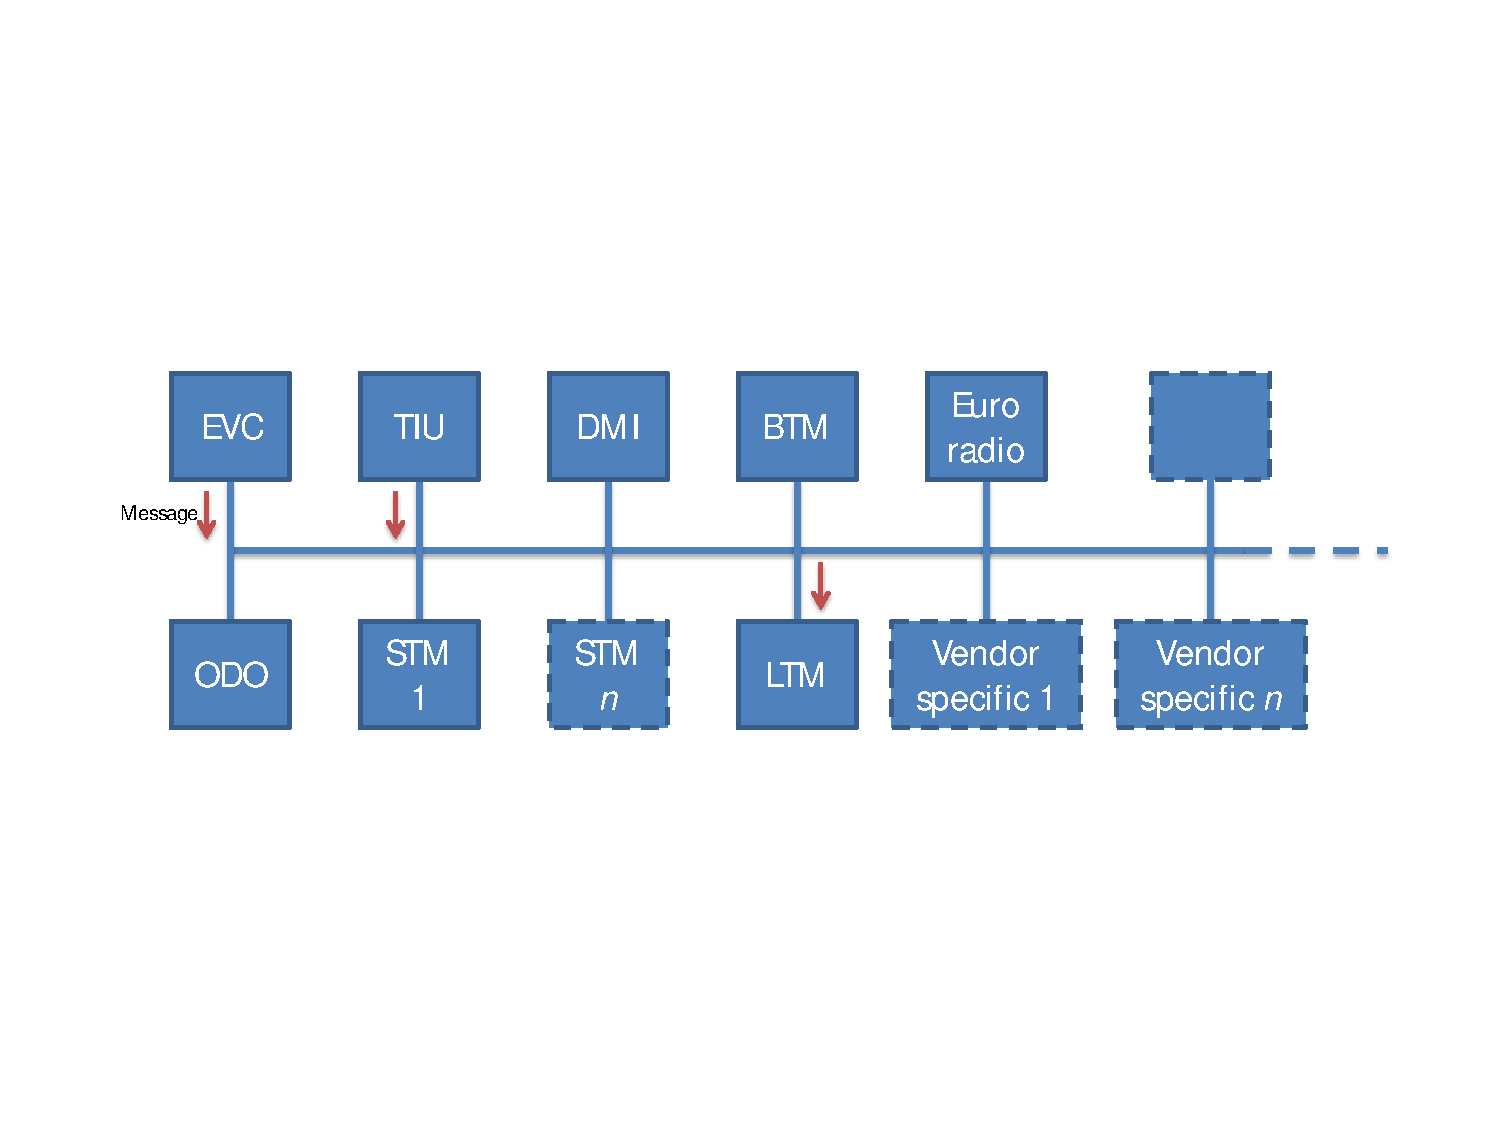
\includegraphics[width=\linewidth]{abstract-hardware-architecture.pdf}
  \caption{Reference abstract hardware architecture}
  \label{fig:hardware-arch}
\end{figure}

The reference abstract hardware architecture is shown in figure
\ref{fig:hardware-arch}.

The reference abstract hardware architecture is made of a bus on which
are connected \define{units}:
\begin{itemize}
\item EVC (European Vital Computer);
\item TIU (Train Interface Unit);
\item ODO (Odometry);
\item DMI (Driver Machine Interface);
\item STM (Specific Transmission Module, up to 8 units);
\item BTM (Balise Transmission Module);
\item LTM (Loop Transmission Module);
\item EURORADIO;
\item JRU (Juridical Recording Unit);
\item Zero or more Vendor specific unit.
\end{itemize}

A given instance of openETCS might not have all of above
units. \FIXME{Define a set of mandatory units?}

Those units shall working concurrently. They shall exchange
information with other units through asynchronous message passing.

% LocalWords:  Alstom openETCS EVC BIU TIU Odometry DMI STM BTM Balise LTM API
% LocalWords:  EURORADIO JRU

\subsection{Reference abstract software architecture}
\label{software-arch}

\subsection{Overall architecture}

\begin{figure}[htbp]
  \centering
  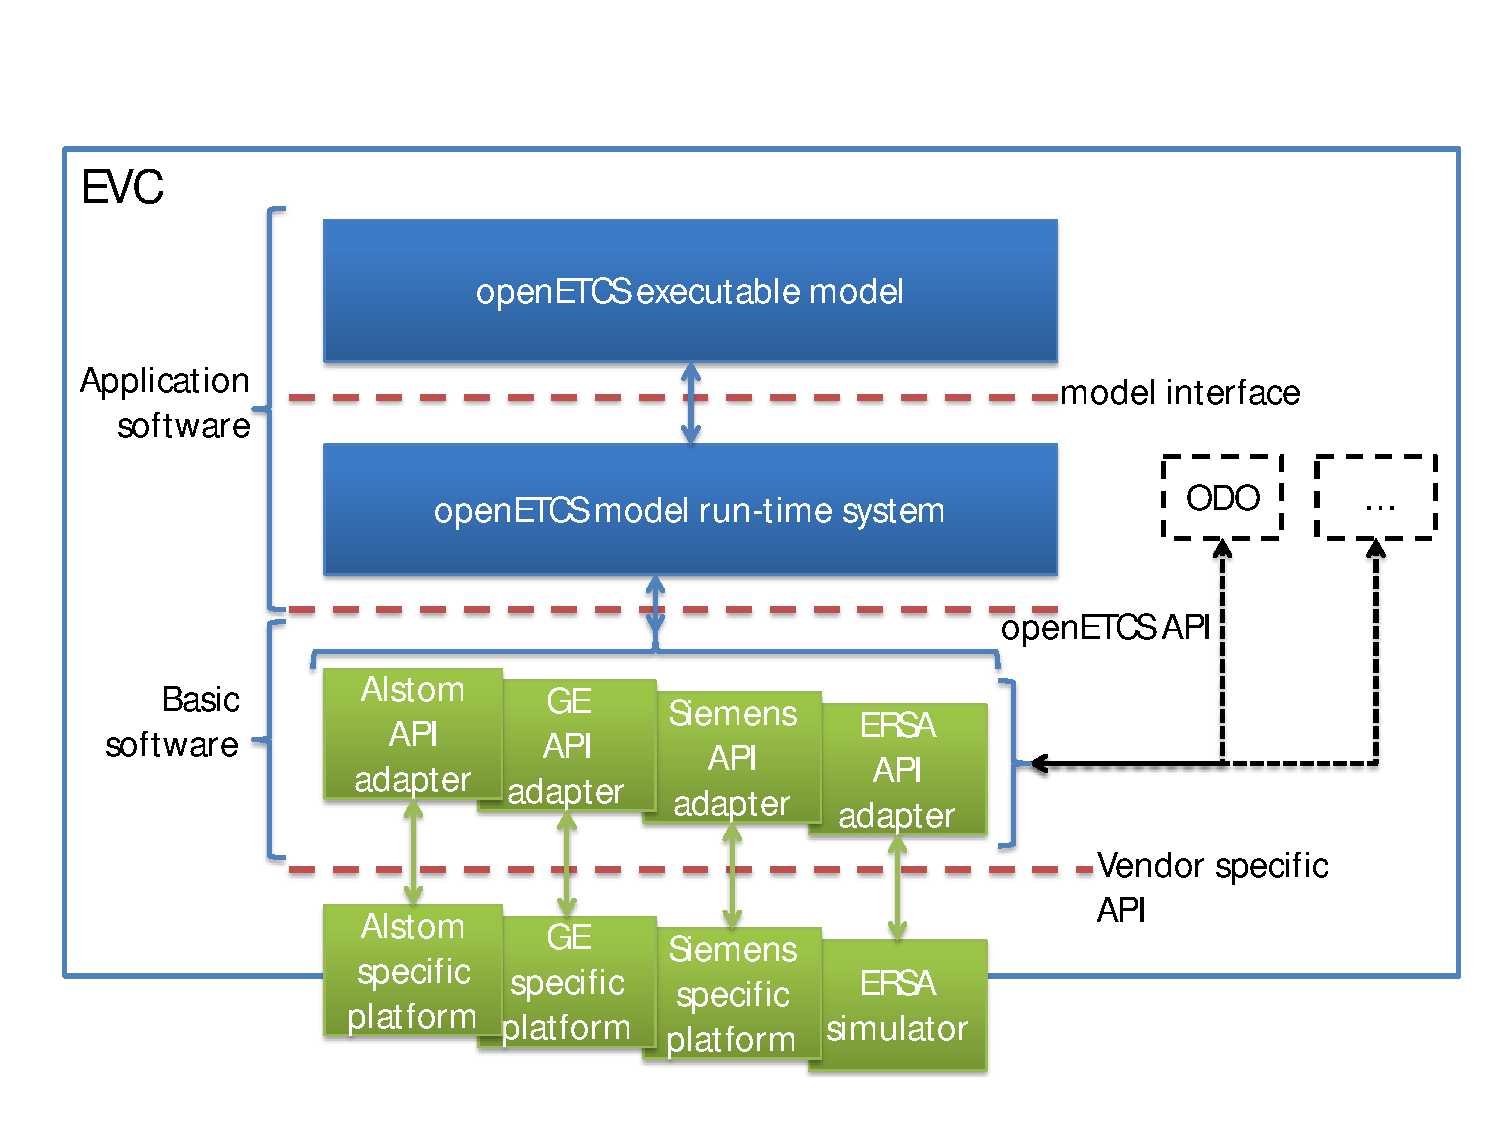
\includegraphics[width=\linewidth]{software-architecture.pdf}
  \caption{Reference abstract software architecture}
  \label{fig:software-arch}
\end{figure}

The \define{reference abstract software architecture} is shown in figure
\ref{fig:software-arch}. This architecture is made of following
elements:
\begin{itemize}
\item \define{openETCS executable model} produced by the
  \cite{scade-model}. It shall contain the program implementing core
  ETCS functions;
\item\define{openETCS model run-time system} shall help the execution
  of the openETCS executable model by providing additional functions
  like encode/decode messages, proper execution of the model through
  appropriate scheduling, re-order or prioritize messages, etc. This
  block shall be described in another openETCS document. \FIXME{ref?}
\item \define{Vendor specific API adapter} shall make the link between
  the Vendor specific platform and the openETCS model run-time system.
  It can buffer message parts, encode/decode messages, route messages
  to other EVC components, etc.
\item All above three elements shall be included in the EVC;
\item \define{Vendor specific platform} shall be all other elements of
  the system, bus and other units, as shown in figure
  \ref{fig:hardware-arch}.
\end{itemize}

We have thus three interfaces:
\begin{itemize}
\item \define{model interface}
 is the interface between openETCS
  executable model and openETCS model run-time system. It shall be
  described in another openETCS document \FIXME{ref?};
\item \define{openETCS API}
 is the interface between openETCS model
  run-time system and Vendor specific API adapter. It is described in
  this document;
\item \define{Vendor specific API}
 is the interface between Vendor
  specific API adapter and Vendor specific platform. This interface is
  not publicly described.
\end{itemize}

The two blocks openETCS executable model and openETCS model run-time
system are making the \define{Application software}
 part. This Application software might be either openETCS reference software or
vendor specific software.

The Vendor specific API adapter is making the \define{Basic software} part.

\subsection{Information exchange between blocks}

At this level of description, we do not explain how the various blocks
of above architecture are calling themselves. We only assume they are
exchanging \define{messages} in an asynchronous way. A message is a set
of information corresponding to an event of a particular unit, e.g. a
balise received from the BTM. The possible kind of messages are
described in chapter \ref{information-flows}.

How the exchange of messages in implemented in actual software,
e.g. function call, storage of data in a shared buffer, ..., is
described in chapter \ref{concrete-interface}.

\subsection{Architectural variations}
Please note that the reference abstract hardware and software
architectures do not forbid architectural variations. For example, the
Odometry function could be put within the EVC (see ODO on figure
\ref{fig:software-arch}) instead of a separate hardware unit (as it
was shown on figure \ref{fig:hardware-arch}). Such Odometry function
would be part of the Application software. But communication between
this Odometry function within EVC and the openETCS model run-time
system shall be done through the openETCS API and shall follow its
conventions.


\subsection{openETCS Model Runtime System}
The openETCS model runtime system also provides:

\begin{itemize}
\item Input Functions From other Units\\
In this entity messages from other connected units are received.
\item Output Functions to other Units\\
The entity writes messages to other connected units.
\item Conversation Functions for Messages (Bitwalker)\\
The conversion function are triggered by Input and Ouput Functions. The main task is to convert input messages from an bit-packed format into logical ETCS messages (the ETCS language) and Output messages from Logical into a bit-packed format. The logical format of the messages is defined for all used types in the openETCS data dictonary. \\
Variable size elements in the Messages are converted to fixed length arrays with an used elements indicator.\\
Optional elements are indicated with an valid flag.
The conversion routines are responsible for checking the data received is valid. If  faults are detected the information is passed to the openETCS executable model for further reaction. 
\item Model Cycle\\
The executable model is called in cycles. In the cycle 
\begin{itemize}
\item First the received input messages are decoded
\item The input data is passed to the executable model in a predefined order. \textbf{(Details for the interface to be defined)}.
\item Output is encoded according to the SRS and passed to the  buffers to the units.
\end{itemize}

\end{itemize}

As another example, part of Vendor specific platform could be on EVC
and thus the Vendor specific API would be within the EVC.

\newpage
\subsection{F1: openETCS API (Input)}
\begin{figure}[hbtp]
\centering
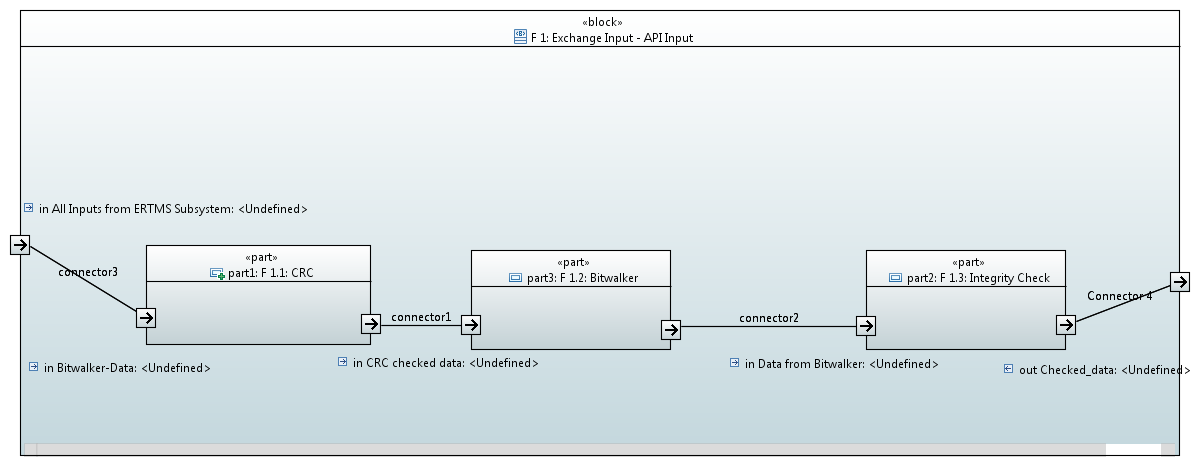
\includegraphics [scale=0.5] {images/F1_Exchange_input}
\caption{Exchange input - API input}
\end{figure}

\textbf{Interfaces aligned with the Alstom API to be added}\\
The exchange input needs to be seperated in 
Basic SW\\
and\\
Application SW \\
since the functions CRC and Bitwalker belong to a basic function. The integrity Check belongs to Application function.\\

\textbf{See Figure 5}\\
 
Inputs:\\
\begin{itemize}
\item TIU
\item DMI
\item BTM
\item EURORADIO
\item ODOMETRY
\item JRU
\item Parameterization board ?
\item Displacement measurement?
\end{itemize}

Outputs:\\
\begin{itemize}
\item The decoded and checked messages from other units are  are output of F1. The information is processed by procedure call provided by the executable model.
\item Details of the granualarity of those interfaces are to be clarified.
\end{itemize}

\section{F1.2: Manage Input}
\begin{figure}[hbtp]
\centering
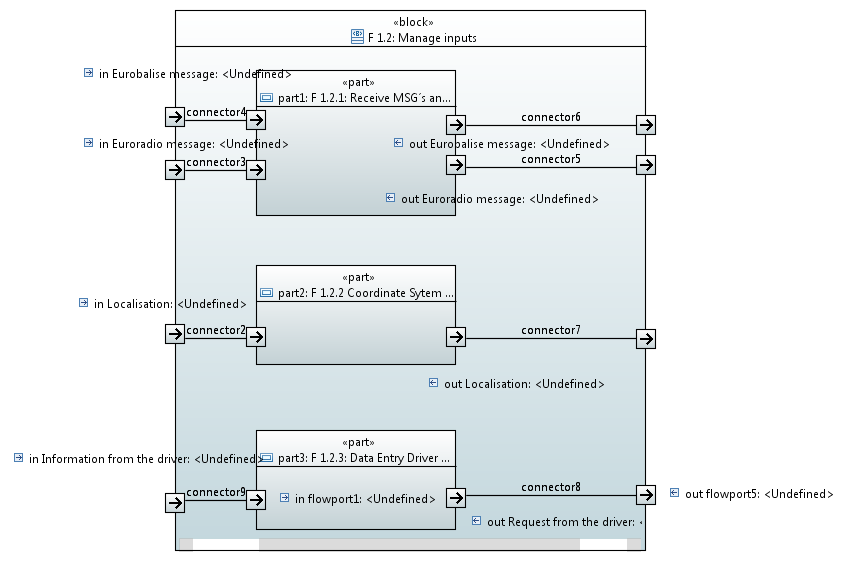
\includegraphics [scale=0.9] {images/Manage_inputs}
\caption{Manage input}
\end{figure}

  Inputs:\\
``will be complete''\\

 Outputs:\\
 ``will be complete''\\
 
 \textbf{ Description:} ???
 
 \newpage
 \section{F1.4: Data structure}
\begin{figure}[hbtp]
\centering
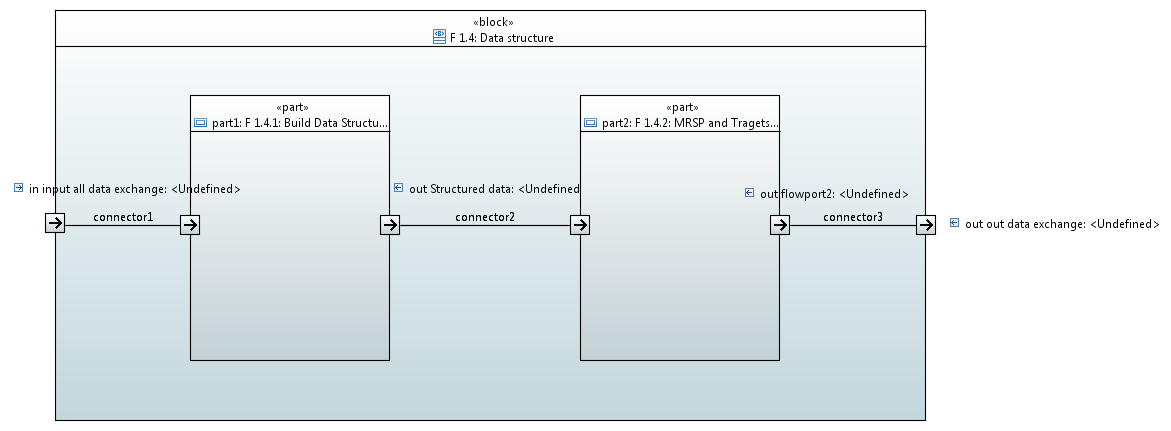
\includegraphics [scale=0.5] {images/data_structure}\\
\caption{data structure}
\end{figure}

  Inputs:\\
``will be complete''\\

 Outputs:\\
 ``will be complete''\\
 
 \textbf{ Description:} ???
 

 \section{F2 Elaboration track messages}
 
 \textbf{See Figure 2 - Block F 2}\\
 
  Inputs:\\
``will be complete''\\

 Outputs:\\
 ``will be complete''\\
 
 Description: This function module provides the encoding and decoding of track messages that 
Management of the port and power off RBC, and the management of reference 
Beacons, which are based on the track messages.\\

 \subsection{	F21: Receive Eurobalise Messages} 
 \textbf{SRS:} § 3.4, § 3.6, § 3.16, § 3.17, § 4.8\\
 
  \textbf{Inputs:}\\
``will be complete''\\

 \textbf{Outputs:}\\
 ``will be complete''\\
 
 \textbf{Description:} 
 This function module provides the summary of telepowering information and the 
review of coherence the content of telepowering message. 
This module separates the eurobalise message as follows: 
 
 - The Balise telegram heads for checking the consistency of the different 
Telegrams, the management of the duplicated beacons and the acquisition of meaning. \\

- Then the information that the balise group, their reading direction and are 
Wegmessungsposition where the first balise group was read, in 
Baliseninformationen for monitoring the function "Manage the eurobalises" 
summarized (see the term Identifzierung and meaning in this function), which the 
Continuation of reading via the information Referenzbalise with a Balisenposition in 
Kernel-reference document approved. \\

\textbf{- The ETCS ETCS version and packages:} \\

The first review is the version ETCS ETCS track with the version Zugbord 
(Version 1.x Class1 =) to compare; these must be compatible (that means 1.y) to 
continue processing (a Balise version of the type is 0.y as incompatible 
considered, but they must not generate a negative reception report). \\

The second review is in compliance with the ETCS grammar in the resulting 
Packets with a packet 255, which terminates the beacon information of each of the group. \\

The reception of a packet 245 (standard package) in a eurobalise) includes the 
Rejection of all other packets received and generated a the same mistake as 
Grammatical errors ETCS, unless the OBU is in Level 2. \\

Only the packets 44, 65, 66 and 136 may be located several times in a same eurobalise message\\ 
For the 136 package: \\
• a single packet 136 per Balise telegram, \\
• the different packages 136 in a same message are identical. \\

The read packets are filtered as a function: \\

- from the direction of the transition to the balise group (the packet is the variable 
QDIR oriented), 
the bi-default state (level, level of announced and ERTMS / ETCS mode). \\

The tables of filtering per level and ERTMS / ETCS mode are in the description of the 
Function "received EUR radio messages" contain.\\

\textbf{These packets are transmitted in four different groups:}

- Geographical information (packet 79 for the "train locations") \\

- Information CNX / DCNX (packets 42, 131) for the "the CNX and DCNX 
Euro Radio Management "\\

- Information Balise (package 136: Referenzbalise for in-fill information) for the function 
"Manage eurobalises" \\

- Track-mail received (other packages) for the "monitor train". \\

\textbf{Any error of Referenzbalise, the version or the grammar ETCS is in CR (radio channel) 
Receiving reported.}\\
 
 
 \subsection{F22: Receive Euroradio Messages}
  \textbf{SRS} § 3.4, § 3.6, § 3.16, § 4.8\\
  
    \textbf{Inputs:}\\
``will be complete''\\

 \textbf{Outputs:}\\
 ``will be complete''\\
 
\textbf{Description:} 
This function module provides the summary of the Euro radio information and the 
Verify the consistency of the contents of the Euro radio message. 
The first guaranteed by this module check is to monitor the radio link. 
This only applies to a normal communication channel (see § 8.3.1 interface gSM-R). \\

\textbf{The review is broken down as follows:}

- Basic principle: the RBC is providing its messages with a time stamp based on the 
Time marking the bi-standard the equipment (if the timestamp of the messages on 
position is undefined, the message is accepted, but only during the initialization of the 
Communication session EVC - RBC).\\

Verification of the sequence: \\

- the ETCS OBU train equipment rejects any message that is "older" than the last 
received message.\\

- the ETCS OBU train equipment is up to any message that is "younger" than the last 
received message.\\
 	 
 	 
\subsection{F23: Manage Eurobalise Messages}
\textbf{SRS} § 3.4, § 3.6, § 3.16\\
  
   \textbf{Inputs:}\\
``will be complete''\\

 \textbf{Outputs:}\\
 ``will be complete''\\
 
\textbf{Description:} 
This function module manages the Balise reference document of the ETCS Onboard Unit, 
is said to know that the information supplied by the track following terms have: \\

- either the balise which provides the information, \\

- or delivered in the radio message Referenzbalise, \\

- or delivered in the infill balise message Referenzbalise (package 136). \\

A balise group contains 1-8 eurobalises. 
The balise group is referenced by an identification NIDLRBG (NIDC: identification 
+ NIDBG region: identification beacon). Each eurobalise has an internal number from 1 to 8, 
which describes the position of the beacon relaltive in the group. \\

A consisting of only one beacon balise group called "simple beacon", as 
any other balise group managed; However, it produces features that described in
Function module F23 and in the function module F25.\\

\subsection{F24: Manage Cnx and Dncx Euroradio}
\textbf{SRS} § 3.5, § 3.15.1, § 5.15\\

 \textbf{Inputs:}\\
``will be complete''\\

 \textbf{Outputs:}\\
 ``will be complete''\\
 
\textbf{Description:} 
This function module ensures the production ending a Euroradio- 
Communication. \\
For the ETCS OBU equipment it is possible to Euro Radio communication session
initiate: \\

- for a "start of mission": train data \\

- after one obtained from the track command: info CNX / DCNX. 
The command, an RBC to contact, the identity of the RBC and its telephone number 
(Packets 42 or 131).\\



 \subsection{F25: Send Euroradio Messages}
 \textbf{§ 3.4, § 3.16}\\
 
  \textbf{Inputs:}\\
``will be complete''\\

 \textbf{Outputs:}\\
 ``will be complete''\\
 
\textbf{Description:} 

This function module ensures the completeness (location and time stamp) and the 
Transmission of radio messages euro on the basis of information "radio session message", 
"Outgoing track message", "message acknowledgment" (for a radio message 136) and "CR 
Radio channel reception "(for a radio message 136 along with a package 4). \\

A radio message is sent only if between the ETCS OBU equipment and the 
RBC opened a euro radio session. \\

The radio messages, with the exception of the message confirmation (radio message 146) and the 
Session messages (radio message 154, 155, 156, 159) contain a "position report" package 
(O or 1 packet). \\

The structure of this "position report" package based on the following information: \\

- Info for locating the data LRBG, position, velocity, position error, moving direction,
by default state for the data concerning the level and the ERTMS / ETCS mode. \\

The package 1 "special position report" is used for one or two LRBG whose 
Crossing direction is not known ((LRBG type simple balise group). \\

The package 0 "position report" is used when the direction of the LRBG is known (group 
not simple beacons, or group simple beacons, whose Balisenrichtung over by the track 
was positioned a link or package 135) (see function F23)).\\
 	
 \textbf{See the functional breakdown of the function in F2 in the next paragraph (Figure 3)}\\
 
\subsection{F2 breakdown}	
 \begin{figure}[hbtp]
\centering
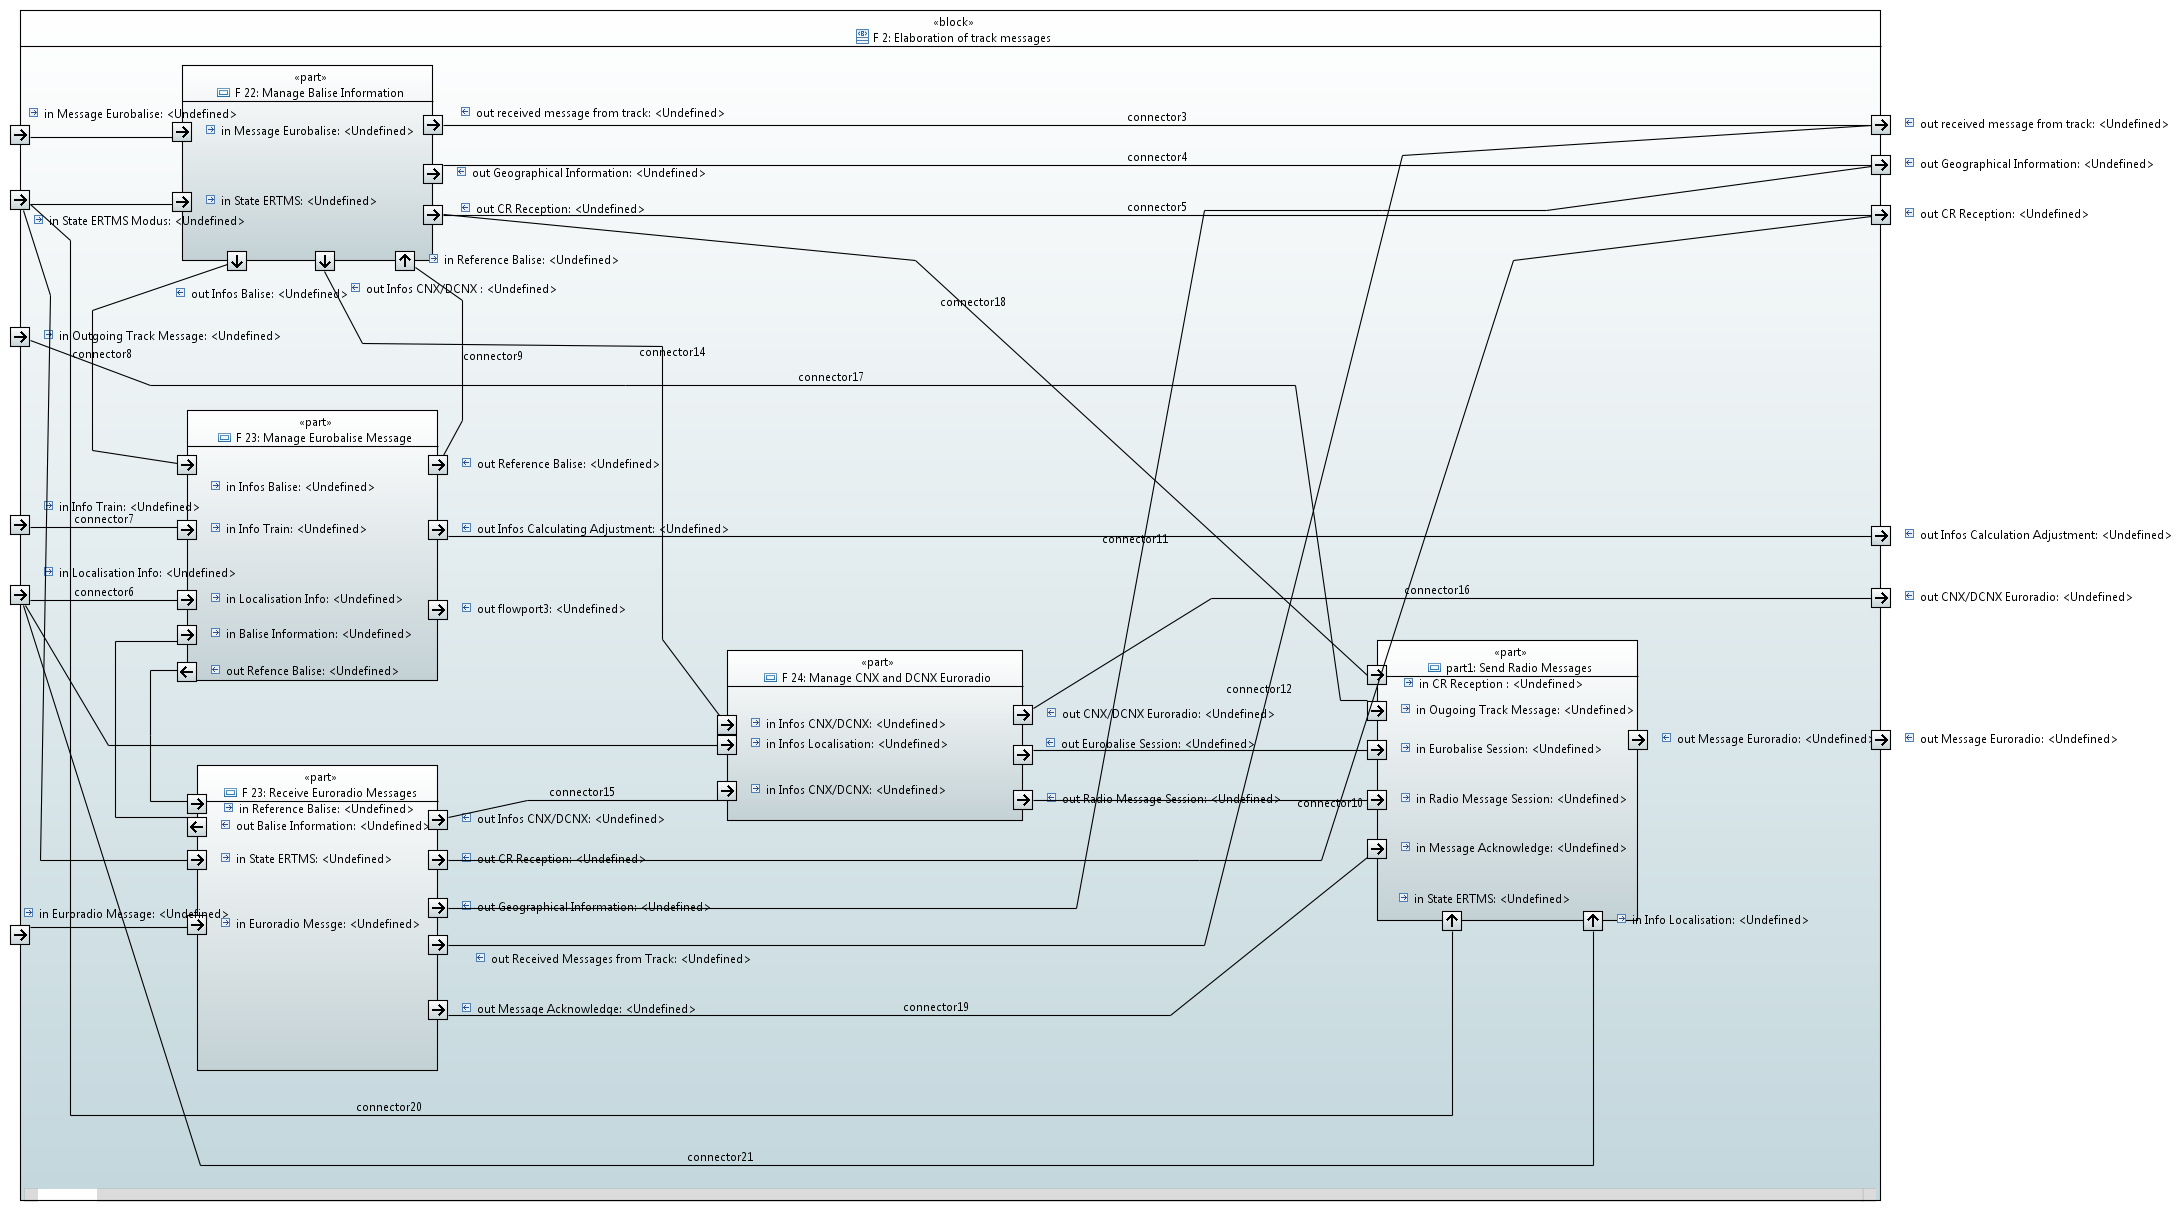
\includegraphics [angle=90, scale=0.3] {images/F2_Breakdown}
\caption{Elaboration track messages breakdown}
\end{figure}

\newpage
\section{F3 Train loction}
\textbf{See Figure 2 - Block F 3}\\

\textbf{SRS} § 3.6.4, § 3.6.5, 3.6.6\\

  \textbf{Inputs:}\\
``will be complete''\\

 \textbf{Outputs:}\\
 ``will be complete''\\
 
\textbf{Description:} 
This function module provides the location of the train in a kernel-reference document 
(Locating information), based on the following reference documents: \\

- path measurement calculation reference documents the function "distance measurement": train location, \\

- Balise the "track messages draw": Information computational comparison.\\


 \section{F4 Train Supervising in ERTMS Modus}
 \textbf{See Figure 2 - Block F 4}\\
 
\textbf{Inputs}:\\
``will be complete''\\
 
 \textbf{Outputs:}\\
 ``will be complete''\\
 
 \textbf{Description:} 
 This function module ensures the monitoring of the train by working out: \\
 
 - The level and mode of control,\\
  
- Monitoring the speed, position and the movement of the train,\\
 
- The driver interfaces,\\
 
The data, which is based on the monitoring.\\

 \subsection {F41: Manage Level ERTMS/ETCS}
 
 \begin{figure}[hbtp]
\centering
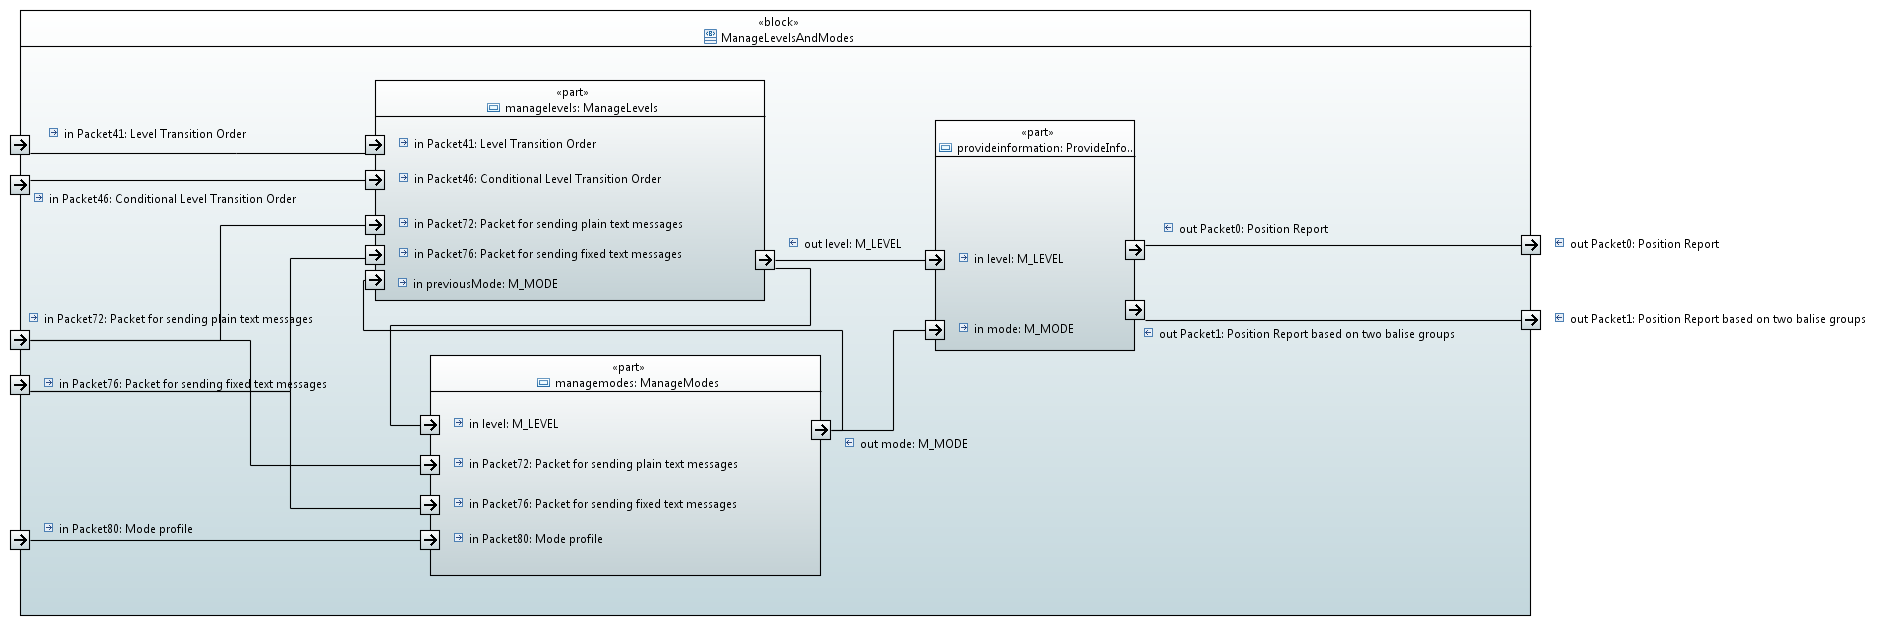
\includegraphics [scale=0.4] {images/Manage_Level_and_Modes}
\caption{Elaboration track messages breakdown}
\end{figure}
 
 \textbf{SRS}§ 5.1, § 3.6.5 \\
 
 \textbf{Inputs}:\\
``will be complete''\\
 
 \textbf{Outputs:}\\
 ``will be complete''\\
 
 \textbf{Description:} 
This function is only applicable for the Eurobalise or Euro radio messages 
announced transitions. The aspect of "use" of the transitions is in Chapter 5 (5.10]
described. \\

This function module manages the transitions of the level ERTMS / ETCS and the 
associated driver acknowledgments and releases associated with these transitions 
related actions. 
The function depends on the current level (managed by this function) and the 
following inputs: \\

- "Get track message": notice the transition, the immediate transition command; \\

- «Info locating": position of the train; \\

- "Request by the driver": acknowledgment of the transition; \\

- «Info train": information exchange of the active driver's cab.\\


 \subsection {F42: Manage Modus ERTMS/ETCS}
 \textbf{SRS}§ 4, § 3.6.5, § 3.15.4, § 5.5, § 5.6, § 5.7, § 5.9, § 5.11, § 5.13 \\
 
 \textbf{Inputs}:\\
``will be complete''\\
 
 \textbf{Outputs:}\\
 ``will be complete''\\
 
 \textbf{Description:} 
description 
This function module manages the transitions of the ERTMS / ETCS mode and the 
associated acknowledgments by the driver, and triggers associated with these transitions 
associated actions. \\

The function depends on the following inputs: \\

 - "Get track message": Adopted train data, SH mode approved indication signal 
(VMAIN = 0), Information «danger for SH" Information "stop if in SR"; \\

- Info locating": train position and indication information; \\

- "Mapper": available allocation to in SR mode, FS, OS or RV 
drive requirement of "train trip" (triggering the train-emergency); \\

-"Request driver»: acknowledgment of the driver 
proposed modes SH and NL, acknowledgment at the end of TR mode, 
Preventing the TR mode; \\

- Info train": TIU Inputs (off, active cab, signal leading / led 
Cab, field monitoring system, condition of equipment; \\

- "ETCS Mode": current mode and current level; \\

- "CR reception": a reported on a balise error or loss of the radio link 
and related response; \\

- "Train protection»: in SH mode Balise prohibited, banned in SR mode Balise 
and the status of theETCS OBU equipment forming equipment (TIU, DMI, 
BTM, Euro radio, board-parameterization, position measurement): any error in the equipment 
(not shown "material flow").\\

\subsection {F43: Train Speed supervision}
 \textbf{SRS}§ 3.7, § 3.8, § 3.10, § 3.11, § 3.12, § 3.13, § 5.7, § 5.8, § 5.9 \\
 
 \textbf{Inputs}:\\
``will be complete''\\
 
 \textbf{Outputs:}\\
 ``will be complete''\\
 
 \textbf{Description:} 
description 
This function module monitors the train speed in comparison to a 
Track assignment / a Movementauthority. \\

You must track the assignment using the information obtained track work out, ie the 
Completeness of the assignment using the information obtained from the track information
concerning MA, check profiles and parameters. \\

\textbf{A complete assignment is based on the following information:} \\

- The radio messages 2 (Approval SR), 3 (​​MA), 33 (MA reference it) and the packages 12 
(MA Level 1), 15 (MA Level 2), 80 (mode profiles), 138 (Reversing area information), 139 
(Reversing supervision information) give information on the approval of 
Movement on the track assignment; \\

- The radio messages 9 (requirement of shortening of MA), 15 (conditional urgent 
Stopping), 18 (refusal of urgent arrest) and 16 packets (repositioning), 
70 (Route Suitability) give the "extensions" of the movement permit information 
concerning the track assignment, that is, that they complement the original track assignment, 
without replacing them; \\

- The radio message 16 (unconditional urgent stop) changes the target point, so 
the train to travel (emergency) passes (equivalent to the train which his 
Has exceeded track assignment); \\

- The packages 21 (Gradientprofil), 27 (velocity profile), 51 (axle load), 65 
(temporary restriction) and 66 (refusal temporary restriction) 
enter the profile information on the track assignment; \\

- The package 57 (MA requirements) are the parameters concerning the track assignment; 
for the technical operation modes, the assignment only to provide information to 
technical mode are limited; \\

- The assignment can also on the position of the train (stop) at the end of a mission, 
a missed beacon or a radio or loss in accordance with the current technical 
Be reduced mode (SRS §4.10). \\

- The package 71 (adhesion factor) called the coefficients of the delay tables 
      Change train (train data service braking and emergency braking): 70\% or 100\%. 
      It should be mentioned that the change of these coefficients by the driver on the 
      ETCS onboard unit is not approved. To ensure interoperability must 
      the application but the "track adhesion" function on the driver 
      manage (see the national value of QNVDRIVERADHES). \\
      
- For mode FS and OS mapping is complete when the gradient profiles and SSP to 
End of the MA are known; Otherwise MA is denied.\\

\subsection {F44: Train Movement supervision}
 \textbf{SRS}§ 3.14 \\
 
 \textbf{Inputs}:\\
``will be complete''\\
 
 \textbf{Outputs:}\\
 ``will be complete''\\
 
 \textbf{Description:} 
This function module supervises train movements, ie it ensures protection against 
the involuntary movements of the train: \\

- Protection against the elopement of the train, \\

- Protection against rolling back of the train, \\

- and monitoring the maintenance of the train. \\

\textbf{This module triggers an unwanted movement of the train from the service brake.} \\

\textbf{Protection against the elopement of the train}\\
The protection against the elopement of the train to avoid the train in one direction 
moves that do not match the current position of the field monitoring of the active driver's cab 
matches. 
This protection is applicable only in SH mode, FS, SR, OS, UN, PT and RV.
If the removal of unwanted motion exceeds the national value DNVROLL, 
The brake is activated. 
When the train goes back again to stop, the brake is by consent of the 
Train driver released. \\

\textbf{Protection against rolling back of the train }\\
The protection against rolling back of the train to avoid the train in the his 
Direction opposite direction, i.e., his current assignment, moved. 
This protection is applicable only in FS mode, SR, OS, PT and RV. 
If the removal of unwanted motion the national value DNVPOTRP for the 
Mode PT and PT and et DNVROLL exceeds for the other modes, the brake is 
activated. When the train goes back again to stop, the brake is by consent of the Train driver released. \\

\textbf{Monitoring the stop of the train }\\
The monitoring of the stop of the train to avoid the train moves, if he in 
SB mode is stationary. 
If the removal of unwanted motion exceeds the national value DNVROLL, 
The brake is activated. 
When the train goes back again to stop, the brake is by consent of the 
Train driver released.\\


\subsection {F45: Train position supervision}
\textbf{SRS} § 3.6.5, 4.4.8, § 4.4.11\\

\textbf{Inputs}:\\
``will be complete''\\
 
 \textbf{Outputs:}\\
 ``will be complete''\\
 
 \textbf{Description:} 
 This function module monitors the trainposition, namely: 

- protection against overshooting the unapproved mode in SH or SR beacons, \\

- and the report "report" the pull position (on the conditions of the train position) to the 
RBC. \\

\textbf{Protection of unauthorized beacons}\\
The protection against overshooting of non-approved mode in SH or SR beacons based 
on the list of approved packages ETCS balise the 49 and 63rd 
This means in each affected mode (SH or SR): \\
 
- if a list was supplied, it contains the list of approved beacons: the 
Driving over a balise not included in this list causes the transition to mode TR 
the ETCS Onboard equipment; \\

- if an empty list is supplied, this means that no beacon is approved: the 
Driving over any Balise causes the transition to mode TR ETCS
On-board equipment; \\

- if no list is supplied, each beacon can be run over. \\


\textbf{position report }\\
At each stop the train in FS mode, OS and SR is systematically a position report on 
a radio message 136 produced. \\

Depending on the requirements of the package 58 ETCS another position report is generated 
("Position report parameters"), i.e. .: \\
 
- a temporary cyclical position report, \\

- a moderate distance zykischer position report, \\

- an immediate position report, \\

- a position report at each crossing a balise group, \\

- a position report at specific locations, ie if the max. Head of the train 
(max safe front end) or the min. End of the train (min safe rear end) a specific 
Has crossed position. \\

- Otherwise, without a request by the track, the position report is limited to each 
Driving over a balise group.\\

\subsection {F46: Data storage}
\textbf{SRS} (§ 4.3), § 3.18\\

\textbf{Inputs}:\\
``will be complete''\\
 
 \textbf{Outputs:}\\
 ``will be complete''\\
 
 \textbf{Description:} 
This function module guarantees the storage of various data in the 
"Train data"; these are then used for the entire function modules of the kernel available (it doesnt show the flow, they are distributed to the total functions).\\
 
\textbf{This train data are broken down as follows:}\\ 

- Parameterization train maintenance; These are the characteristics of the train and the track 
(Train data, fixed data and otherwise national standard data),\\
 
- Additional data; these are the data of the mission of the train. \\

The additional data from the driver at the end of the process "start of mission» 
adopted (see function "with the driver dialoguing) and § 6.3 procedure 
"Start Of Mission). This validates the additional data and allows the validation of the beginning 
a mission. \\

See § 4.3 DATA for details of the data. \\
The train data are sent over a track auszusendende message to the RBC 
(Radio message 129, Parcel 11). 
The data obtained from the track national values ​​(Package 3) will be stored and 
considered when the track region (NIDC the Balise of locating information) in one of the 
received national values ​​specified region.\\

\subsection {F47: Dialog with the driver}
\textbf{SRS} § 5.4, § 3.12.3\\

\textbf{Inputs}:\\
``will be complete''\\
 
 \textbf{Outputs:}\\
 ``will be complete''\\
 
 \textbf{Description:} 
This function module ensures the dialogue with the driver at a start 
a mission and for all on-board advertisements (messages, symbols, dynamic data) and the track 
Text messages. \\

The method "start of mission" consists in starting or restarting (end of mission 
the train) for a new mission. \\

\textbf{See Chapter 5 for the method "start of mission."} \\

- The track text message is a resulting free track text message (packet 72) with display and
Display end conditions that are dependent: \\
    • Level of ERTMS / ETCS, \\
    • mode of ERTMS / ETCS, \\
    • from a distance, \\
    • from one time interval, \\ 
    • of an acknowledgment by the driver. \\
The condition can be single or multiple (combination of multiple conditions). 
In the case of the expectation of an acknowledgment by the driver at the end of other 
Combined display conditions, and if these are met, the managed Eurocab- 
Board equipment service braking (lack of acknowledgment). \\

A resulting encoded text message (packet 76) generates an error message because the text codes 
are not defined. \\

The track text messages and the driver displays are in messages 
summarized, which are intended for the DMI: dynamic message (coming from the KV 
Information) symbols and train-text messages. \\

The train-text messages are managed by internal text codes that the DMI an ad in 
chosen by the driver language enable (choice at the beginning of the "start of 
mission "or during the mission).\\

\subsection {F48: Manage brake controll}
\textbf{SRS} § 3.14.1\\

\textbf{Inputs}:\\
``will be complete''\\
 
 \textbf{Outputs:}\\
 ``will be complete''\\
 
 \textbf{Description:} 
This function module ensures the release of the brake control (output 
"Brake control"). \\

The allowances are as follows: \\
 
 - The technical TR and SF mode (input "State ETCS") produce a 
emergency braking, \\

- The lack of acknowledgment of the level, the mode or text message (input 
"Lack of acknowledgment") causes a braking operation, \\

- The protection of the train by the movement monitoring (input "train protection") causes a 
Service braking \\

- FS a reaction to a Bali mustard Ehlers or a wireless loss (input "CR 
Receiving "causes a braking operation, \\

- The direction indicated by the speed monitoring overspeed FS or FU 
(Input "overspeed") causes an operating or emergency braking. \\

Each service brake application (except for overspeed) is an emergency braking 
replaced when the service brake: \\

- Does not exist (train data), \\

- Not after the brake reaction time (train data) after reading the service brake (input 
"Info train") is not working. \\

The solution braking is managed by the requesting functionalities (at a 
Change the mode or the rectification of the fault).\\

\subsection {F49: Manage Train Control}
\textbf{SRS} § 3.12.1, FFFIS TIU\\

\textbf{Inputs}:\\
``will be complete''\\
 
 \textbf{Outputs:}\\
 ``will be complete''\\
 
 \textbf{Description:} 
This function module ensures the development of the using of the train control: \\

- to Control: service brake or emergency brake\\

- the resulting track message "tracks conditions" (Package 68) \\

- the resulting track message "track condition big metal masses" (Package 67) \\

- the resulting track message "linking", which allows a calibration range to 
define (Package 5). \\

The drafting of "track conditions" and the "calibration range" is national in § 4.4 
And functions described in § 4.5. The "track conditions" (Package 68) activate the corresponding train control systems and give them 
the driver to. The package 68 provides the start and end of the "tracks 
conditions ". \\
The "big metal masses track condition" (Package 67) puts the transmission in BTM state 
OFF. \\
This causes the disruption of the broadcast antenna of the ETCS onboard equipment. 
The package 67 provides the beginning and end of the track condition "big metal masses." 
At the end of this condition in the transmission mode is "not modulated", so the the 
Default is to read the eurobalises. \\

There is a manual calibration of the measurement system exists, it is, however, directly from the 
Linear Position Sensing subsystem through the acquisition of the Wegmessungsdaten 
Bordparametrierungsmoduls managed. 
However, the bi-standard onboard equipment is capable of automatic calibration ranges of 
To capture Bordwegmessungssystems: 
A calibration range is announced between two Eurobalisegruppen 
Calibration area having the following properties: \\
     • Distance between the Euro balise 'groups greater than 1000m, \\
     • Linking error between the Euro balise 'groups smaller than 1 m, \\
     • Gradientprofil between the eurobalises, the closest to a zero-gradient 
         are, \\
     • Travel between the beacons with a least possible number of curves. \\
Therefore, these properties are the responsibility of implementing this track 
Areas, but the first two conditions are those of the ETCS onboard equipment 
allow to detect a calibration area.\\


 \subsection{F4 breakdown}	
 \begin{figure}[hbtp]
\centering
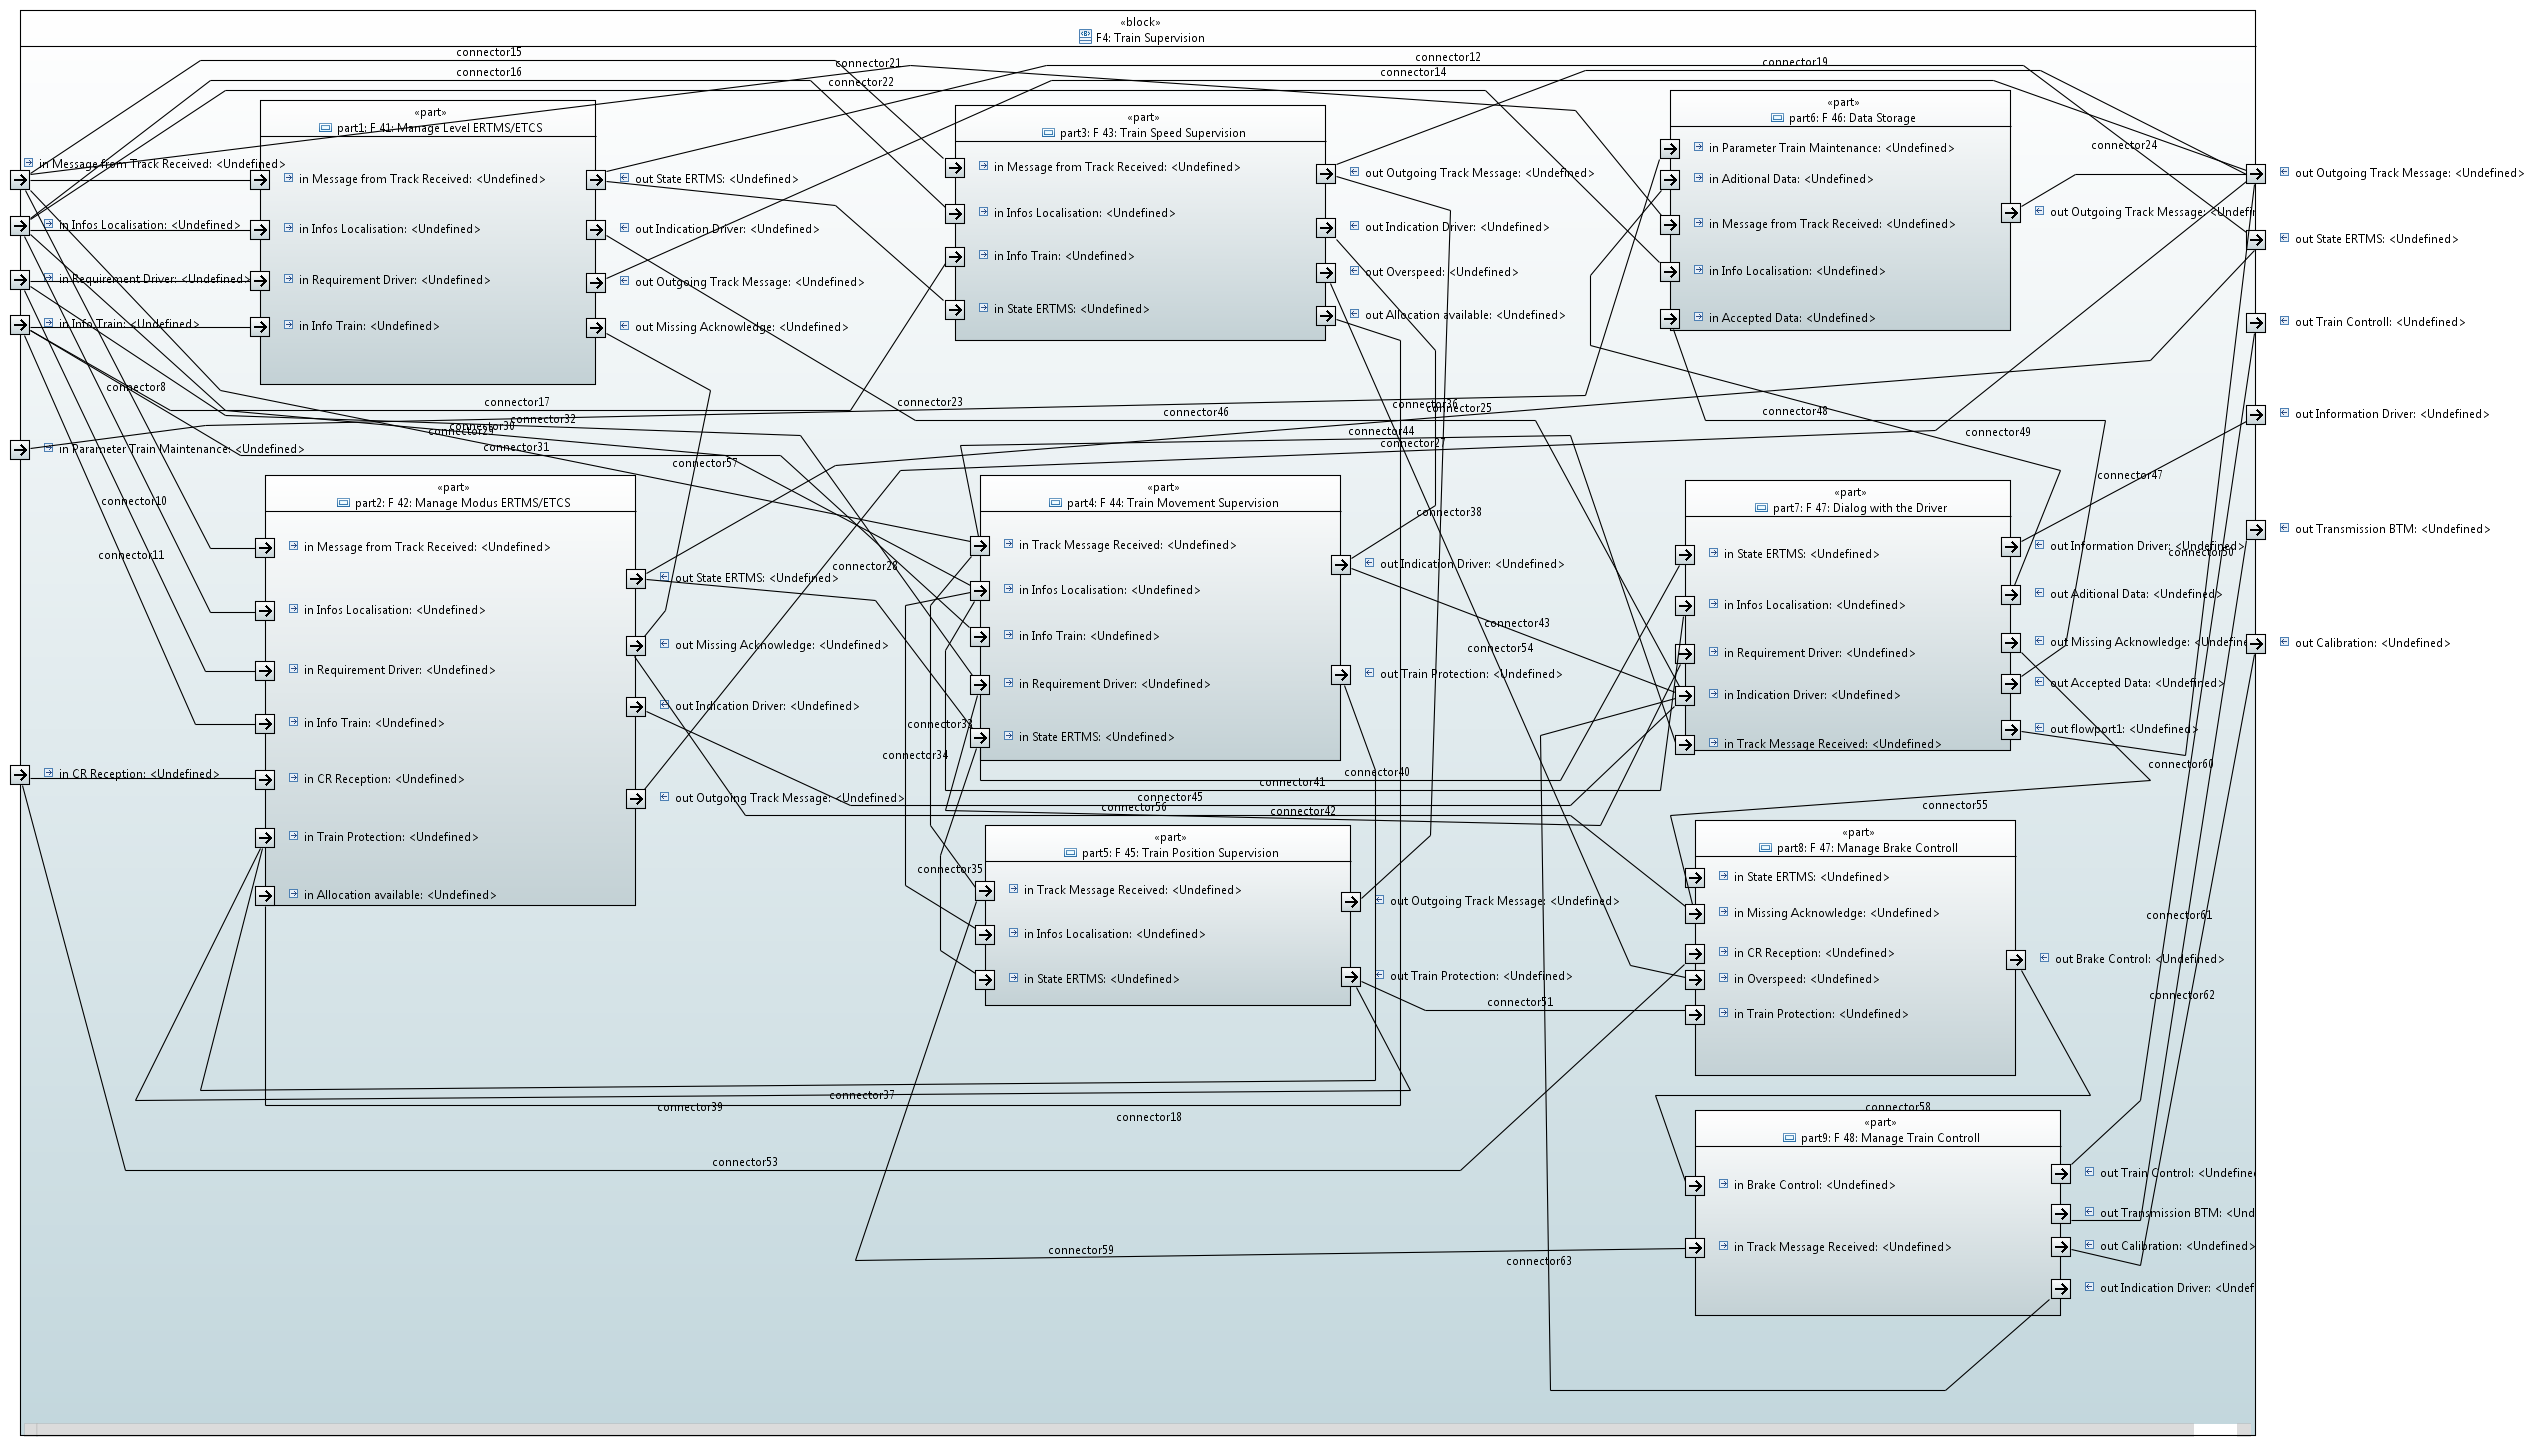
\includegraphics [angle=90, scale=0.25] {images/F4_Breakdown}
\caption{Train Supervising in ERTMS Modus}
\end{figure}

\newpage

 \subsection{F5 Exchange outpout}

 \textbf{ See Figure 2 - Block F 5}\\
 
 \textbf{Inputs}:\\
``will be complete''\\
 
 \textbf{Outputs:}\\
 ``will be complete''\\
 
 \textbf{Description:} 
 description 
This function module manages the exchange at the output of the ETCS On board equipment with 
the following modules: 

- TIU, \\
- DMI, \\
- BTM, \\
- EURORADIO,\\ 
- SAM, \\
- Displacement measurement. \\

It complements their functions at the level of exchange protocols and the "safety layer" for 
the entire module with the exception of Wegmessungsmoduls (that manages its own 
Exchange protocols). 
Note: The manner in which these functions are implemented, is free; the 
details of which are specified in the software specification documents.\\
 
\chapter{Data Flow Description}

\section{List of Data FlowsID}
\tablehead{
\hline 
\rowcolor{gray} 
Number & Flow & Source/Sink & Description  \\\hline}
\begin{supertabular}{| m{3,5cm} | m{3,5cm} | m{3,5cm} | m{3,5cm} |}
1.0 & Missing Acknowledge & Kernel xx/Kernel xx & This information indicates the absence of the 
Acknowledgment of the driver to a 
confirmatory text message on the Level 
Transition, the transition mode or a track 
Train-text message\\\hline
2.0 & Acknowledge & Kernel xx/Kernel xx & Radio message 146 transmission Confirmation - Confirmation message depending on the variable 
§ 8.6.7  \\\hline
3.0 & Action Driver & Kernel xx/Kernel xx &  Election / confirmation / detection Driver via DMI \\\hline
4.0 & Display Driver & Kernel xx/Kernel xx & For the driver specific DMI display \\\hline
5.0 & Reference Balise & Kernel xx/Kernel xx & information; in the Flow "information Balise"  delivered Balise confirmed as a reference beacon.\\\hline
6.0 & Allocation available & Kernel xx/Kernel xx & Information message that an allocation for a given technical mode is available.\\\hline
7.0 & Calibration & Kernel xx/Kernel xx & Specifying a calibration range of the 
path measurement.\\\hline
8.0 & Cnx/Dcnx Euroradio & Kernel xx/Kernel xx & Command on the connection and disconnection of a 
or of a RBC, the identity and 
Phone RBC contains.\\\hline
9.0 & Brake Controll & Kernel xx/Kernel xx & Control of the service and the 
emergency braking. \\\hline
10.0 & Train Controll (brake) & Kernel xx/Kernel xx & Functional output.\\\hline
11.0 & CR Reception (Radio Channel) & Kernel xx/Kernel xx & CR (radio channel) on receipt of a balise or 
Radio message: Checking version ETCS, 
Grammar ETCS, testing reference balise 
(Position), monitoring radio link\\\hline
12.0 & Accepted Data & Kernel xx/Kernel xx & Information valid confirmation of the train data and 
Consequently, at the very beginning of the mission.\\\hline
13.0 & Additional Data & Kernel xx/Kernel xx & Data relating to the mission of the train: 
Identity of the driver, 
selected level, identity and mandatory. of the RBC, 
if Level 2, no. Mission\\\hline
14.0 & JRU Data & Kernel xx/Kernel xx & Recorded legal data.\\\hline
15.0 & Input Train & Kernel xx/Kernel xx & From the train coming TOR digital inputs and 
Digital outputs \\\hline
16.0 & State ERTMS & Kernel xx/Kernel & Current Level and operating mode ERTMS, announced ERTMS Level and Current Level and operating mode ERTMS, announced ERTMS Level\\\hline
17.0 & Indication Driver & Kernel xx/Kernel xx & each specific for the driver 
Specification. This includes the dynamic information 
speed monitoring the 
different messages and symbols, the 
Exchange during the "start of mission"\\\hline
18.0 & Info Train & Kernel xx/Kernel xx & From Train comming functional information TIU \\\hline
19.0 & Message Eurobalise & Kernel xx/Kernel xx & Information, which the ID 
Balise group (country ID + ID 
Balise), their reading direction and their 
Contains path measurement for review 
(see Flow "reference balise")\\\hline
20.0 & Information cnx/dcnx & Kernel xx/Kernel xx & Information identifying the RBC ID 
(Identification of land + the identification of the RBC), 
RBC his phone number and the authorization \\\hline
21.0 & Information Driver & Kernel xx/Kernel xx & Specific for the driver 
Function DMI information. They contain the 
different specifications for the 
Driver, which are generated from the 
different Function modules.\\\hline
22.0 & Geographical information & Kernel xx/Kernel xx & Absolute current position of the train, which the 
add the flow "location information" \\\hline
23.0 & Information Localisation & Kernel xx/Kernel xx & Locating the train: position and speed of the train in the 
different reference documents, 
including the absolute geographical 
Position.\\\hline
24.0 & Message Eurobalise & Kernel xx/Kernel xx & Flow, summarizing the message / messages eurobalise. 
BTM to F1: the entire telegrams 
F1 to F2: Message 
(the safety layer and the 
the safety layer and the transfer of 
Telegrams in a message by F1 
F1 guaranteed)\\\hline
25.0 & Infos Calculation Adjustment & Kernel xx/Kernel xx & Information, which contains the ID 
Balise group (country ID + ID 
Balise), their path measurement and her for the 
computational comparison of the on-board 
Contains reference document expected position\\\hline
26.0 & Localisation Train (ODO) & Kernel xx/Kernel xx & path measurement in comparison to a 
Balise (+ safety margin), Speed ​​(+ 
Safety distance), direction of travel and capture 
of stopping\\\hline
27.0 & Euroradio Message (train to track) & Kernel xx/Kernel xx & Transmitted Euro radio message 
(the safety layer is guaranteed by F5)\\\hline
28.0 & Euroradio Message (track to train) & Kernel xx/Kernel xx & Received Euro radio message 
(the safety layer is guaranteed by F1)\\\hline
29.0 & Radio Message Session & Kernel xx/Kernel xx & Message / parcel Euro Radio for creating and 
Termination of the radio connection\\\hline
30.0 & Outgoing Track Message & Kernel xx/Kernel xx & Before Inform creation and timestamp 
(except the message flow 
Radio link, message confirmation and CR 
Reception) sent to the track to 
function message\\\hline
31.0 & Message from Track Received & Kernel xx/Kernel xx & Via radio or beacon message received function 
(except the Riverside current 
Information, cnx / dcnx information, Balise 
information)\\\hline
32.0 & Parameter Train maintenance & Kernel xx/Kernel xx & Fixed data, train data, domestic values\\\hline
33.0 & Train Protection & Kernel xx/Kernel xx & Information, protection against rolling 
Twitching, monitoring of stopping, the 
Transition to an unauthorized Balise in SH 
or SR reports\\\hline
34.0 & Balise Reception & Kernel xx/Kernel xx & Information of receipt of a reference Balise NPIG = 0 from the associated type for the computational comparison of the displacement measurement\\\hline
35.0 & Requirement Driver & Kernel xx/Kernel xx & By driver outbound (see flow 
"Action Driver") or from DMI DMI produced 
function information\\\hline
36.0 & Euroradio Session & Kernel xx/Kernel xx & State of the Euroradio connection \\\hline
37.0 & Signal Eurobalise & Kernel xx/Kernel xx & Airgap Eurbalise -> BTM\\\hline
38.0 & Signal Euroradio & Kernel xx/Kernel xx & Airgab RBC ->Euroradio Board\\\hline
39.0 & Output Train & Kernel xx/Kernel xx & Train digital outuputs\\\hline
40.0 & Overspeed & Kernel xx/Kernel xx & Information message overspeed
of the train relative to the
speed curves\\\hline
41.0 & Synchronization & Kernel xx/Kernel xx & Synchronization (xw, V, T) between the kernel, 
the BTM and the path measurement\\\hline
42.0 & Transmission BTM & Kernel xx/Kernel xx & Control BTM - antenna\\\hline
\end{supertabular}

\chapter{Functional and data structure architecture ETCS on-board} \label{sss:functionaldatastructure}
 Within the following chapter Description of Functional and data structure architecture ETCS on-board the datastrucutre is explained and detailed on location based data.
\FIXME{To be considered and merged to the overall architecture view!!}

%%% Local Variables: 
%%% mode: latex
%%% TeX-master: t
%%% End: 

\section{Data Structures} \label{ss:datascructures}
\subsection{Introduction}
The data flows and data structures used in the application are the interface between the functional blocks. A clear definition of the data will allow sharing the workload between different groups without causing too much communication overhead. The data structures are part of the \textbf{Data Dictionary}.

Data can be distinguished in data storage which is remembered as a system state: “data stored on-board” see SUBSET-026-A.3.4, and data temporarily stored.


Data structures shall be designed for:

\FIXME{API Synchronization}
Inputs (to be synchronised with the API specification):
\begin{itemize}
\item structures for messages
\item data from other inputs: odometer, DMI, TIU, STM's
\end{itemize}

\FIXME{API Synchronization}
Outputs (to be synchronised with the API specification):
\begin{itemize}
\item structures for output messages
\item data to other outputs: DMI, TIU/BIU, STM's, JRU (not including technical communication, like distributing the system time)
\end{itemize}


\subsection{Data structures to store received messages}
Messages are received either by Euroradio or Eurobalise (Euroloop is not yet taken into account). The Euroradio will provide a message in one block of data, from a Eurobalise Telegrams (the part of a message sent by one balise) are received, which have to be put together into a message.

Eurobalise Messages contain a header to give the following information:
\FIXME{Needs synchronization according to SUBSET-026-8.4.2.1}
\begin{itemize}
\item valid version of ERTMS/ETCS system
\item \verb+NID_BG+ identifier of the BG 
\item \verb+NID_C+ identifier of the country
\item reference to which information is given (identifier of the LRBG), in case of a radio message.
\item information for constructing the message out of the Telegrams and for checking message consistency (balise numbering, message counter, duplicate information etc.)
\end{itemize}

Euroradio Messages contain a header to give the following information:
\FIXME{Needs synchronization according to SUBSET-026-8.4.4.6.1}
\begin{itemize}

\item \verb+NID_MESSAGE+ - identifying the message number
\item \verb+L_MESSAGE+ - Message length including everything from field 1 to padding inclusive
\item \verb+T_TRAIN+ - Time Stamp from RBC
\item \verb+M_ACK+ - Inidicating of the message must be acknowledged
\item \verb+NID_LRBG+ - identifying the  
\item further variables as required by \verb+NID_MESSAGE+
\end{itemize}

The message header is used to check the consistency, to check if the message is valid for the current direction, define the reference for location based data and construct the message out of Telegrams.

Further messages contain “packets” as defined in SUBSET-026 chapter 7. 

Radio-messages are received as a bit stream in a minimised data format. To allow efficient processing the data has to stored using standard data-types (fixed point) in structures for individual packets. The chain of components between receiving the message from the antenna to storing packets using standard types is:
\FIXME{needs a design decision - consistent with high level architecture?}
radio - EVC basic software – bit walker – filtering.
Functions are assigned as follows to the different modules and functional blocks:
\begin{itemize}
\item CRC checking shall be done in the radio. The result of the CRC check shall be made available for the application software.
\FIXME{Exact definition of CRC error needs to be added here} (because a CRC error is to handled by the application as a consistency error, i.e. “linking reaction”).
\item Translating the bit stream into variables of a standard (fixed point) data-type and store the data in a memory accessible by the application software. The way the data stream has to be put into variables and stored depends on the version of the track-side ETCS installation. (see \verb+M_VERSION+ and SUBSET-026-6)
Indexes (``pointers'') shall be set to packets contained in the message, i.e. an array containing  the indexes of the first packet of a certain type. The array shall have one element per possible packet. Each packet shall have an extra field to refer to the next packet of the same type in the message (only possible for a few packet types).
This shall be done by the “bit walker”.
\item Detecting the version of the track-side ETCS system is to be handled in the application.
\item Check on illegal values in the packets. (if detected, set a flag for “consistency error”).
\item Couple the location reference to the different packets (those can be different for different packets in case infill information is included in the message, i.e. all packets after packet 136 contain infill information (have to be reference to the LRBG using linking information).
\item Translate the identity of the location reference (a BG) from \verb+NID_BG+ to the index and array where the concerning information is stored.
\item Check if the packets have to be taken into account or have to be stored in a transition buffer according to the current mode and level (filtering) and mark the packets if they shall be used.
\end{itemize}

To facilitate the above described functions, a data structure is necessary capable of storing at least 2 complete messages plus extra variables to store the result of CRC checking and the check on illegal values. Further for each packet variables are needed to store the reference position for the information in the packet (\verb+NID_BG+ and index plus array where the BG information is stored). In addition an array is needed to store “pointers” to the start of each packet in the message.



\begin{figure}[ht]
\centering
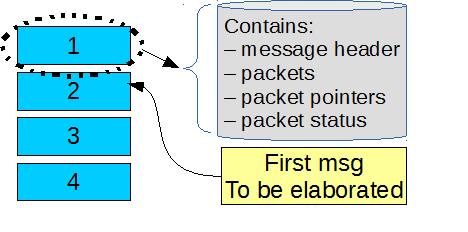
\includegraphics[scale=0.6]{../images/DataStructure_NotYetElaboratedMessages.png}
\caption{Data structure to store not yet elaborated messages.}\label{fig:DataStructureTelegramStructure}
\end{figure}


Data structure to store not yet elaborated messages as found in figure \ref{fig:DataStructureTelegramStructure} are further described in \ref{fig:SingleElementLocationBasedDataStructure} and \ref{fig:SingleElementLocationBasedDataStructure}. A special value for the ``pointer'' is defined for the case no radio messages are available.
Further pointers to the individual packets are required for efficient elaboration later on. 

The different functions can work on the same data structure, i.e. the structure is filled once and is than used up to the point where the packets are elaborated.


Eurobalise (BTM) -messages are received as a bit stream in a minimised data format per balise telegram. To allow efficient processing the data has to be stored using standard data-types (fixed point) in structures for individual packets. The chain of components between receiving the message from the antenna to storing packets using standard types is:
BTM - EVC basic software – bit walker – filtering.

\FIXME{needs a design decision - chain of components consistent with high level architecture?}
Functions are assigned as follows to the different modules and functional blocks:
\FIXME{CRC checking to be better described}
\begin{itemize}
\item CRC checking shall be done in the BTM per Telegram. The result of the CRC check shall be made available for the application software (because a CRC error is to handled by the application as a consistency error, i.e. “linking reaction”).
\item Translating the bit stream into variables of a standard (fixed point) data-type and store the data in a memory accessible by the application software . If there is already a Telegram from the same balise stored and depending on the message counter of the telegram header, the new data shall overwrite that Telegram. The way the data has to be stored depends on the version of the track-side ETCS installation.
\item “Pointers” shall be set to packets contained in the message, i.e. an array containing  the indexes of the first packet of a certain type. The array shall have one element per possible packet. Each packet shall have an extra field to refer to the next packet of the same type in the message (only possible for a few packet types).
This shall be done by the “bit walker”.
\item Detect the version of the track-side ETCS system, to be done in the application.
\item Check on illegal values in the packets. (if detected, set a flag for “consistency error”).
\item Couple the location reference to the different packets (those can be different for different packets in case infill information is included in the message, i.e. all packets after packet 136 contain infill information.
\item Compose a message out of the Telegrams if a balise of another BG is found, if all balises of a BG are found, if the maximum distance (12m) since the last detected balise has been passed.
\item Gather the BG information needed to build the “reference (coordinate) system”.
\item Translate the identity of the location reference (a BG) from \verb+NID_BG+ to the index and array where the concerning information is stored, see figure \ref{fig:DataStructureLocationBasedData}.
\item Check if the packets have to be taken into account or have to be stored in a transition buffer according to the current mode and level (filtering) and mark the packets if they shall be used.
\end{itemize}

\FIXME{what is the rationale behind only storing 15 telegrams?}

To facilitate the above described functions, a data structure is necessary capable of storing at least 15 telegrams plus extra variables to store the result of CRC checking and the check on illegal values. Indexes (“pointers”) indicating where the information of a completed message can be found shall be set. BG information (location, the identity of the BG, etc.) has to be stored in a separate structure for further evaluation. Further for each packet variables are needed to store the reference position for the information in the packet (\verb+NID_BG+ and index plus array where the BG information is stored). In addition an array is needed to store “pointers” to the start of each packet in the message.


\begin{figure}[ht]
\centering
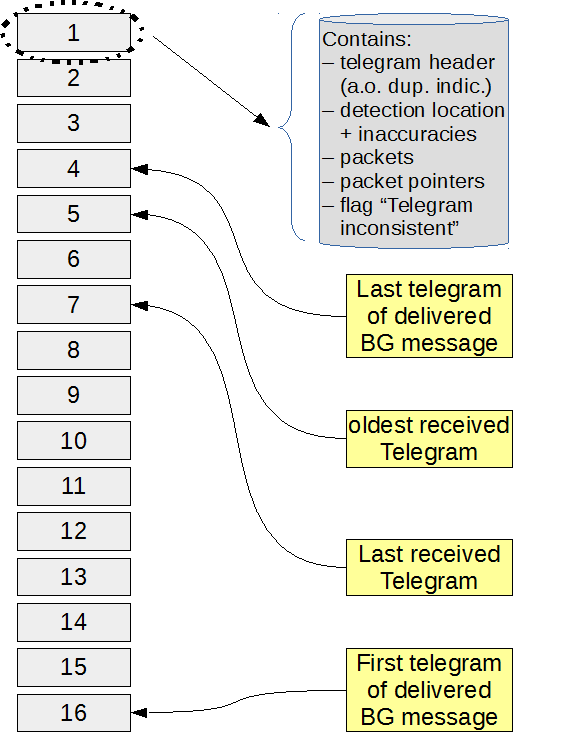
\includegraphics[scale=0.6]{../images/DataStructure_TelegramStructure.png}
\caption{“Telegram structure”: Structure in which Telegrams shall be stored by the “bit walker”.}\label{fig:DataStructureTelegramStructure}
\end{figure}



A completed message can during the consistency check and the check on linking, be kept in the same structure.

In the example shown in figure \ref{fig:DataStructureTelegramStructure}:
\begin{itemize}
\item A message is just made available consisting of 5 telegrams stored at position 16, 1,..,4.
If no message is available the pointers \textbf{``last telegram of delivered BG message''} and \textbf{``First telegram of delivered BG message''} message have a special value. After elaboration of the message and retrieving the packets (done in the same cycle) the pointers will be reset to this special value
\item Since receiving the last Telegram of the delivered message, 3 more (5, 6, 7) Telegrams were detected.
\item \textbf{“Oldest received Telegram”}: the oldest Telegram stored by the “bit walker” which has not been used in a completed message. If no Telegram is waiting for the completion of a BG-message the “pointer” shall have a special value.
\item \textbf{“Last received Telegram”}: the last Telegram stored by the “bit walker”. If no Telegram is waiting for the completion of a BG-message the “pointer” shall have a special value.
\end{itemize}


For packages which are not yet to be taken into account a data structure has to be designed to store the packages for later use inside the \textbf{``transition buffer''}. The stored packages shall be elaborated if the mode and level for which they are stored is reached (generic condition or shall those be stored with the packet).
The minimum number of packages which could have to be remembered, i.e. the minimum storage capacity to be reserved, is to be determined.
\FIXME{determine minimum packages to be remembered within the transition buffer}

\subsection{Data structures to store input data from other sources}

Other input data:
\begin{itemize}
\item TIU: Isolation, brake status (commanded, pressure, inhibited,...)
\FIXME{to be completed}
\item DMI: data-entry, acknowledgements, etc. 
\FIXME{to be completed}
\item STM's: out of scope for the current project. 
\end{itemize}

TIU
The data coming from the TIU is wrapped up in SUBSET-034 and needs amendments for the specific use of the OBU inside a locomotive. A data structure for storing all possible information shall be designed.
\FIXME{complete design of TIU related  data}

DMI
The data coming from the DMI, consists of inputs required based on information sent to the DMI in the context of a procedure.



\subsection{Data structures for “data stored on-board”}
This section is independent to the fact that what happens if the OBU is switched off
\FIXME{data stored on board needs to be completed}
\begin{enumerate}
\item Location based data (a.o. announced BG's, SSP, speed restrictions, location based level transitions, text messages,..)
\item Actual MRSP and list of targets as a distance from the trains front end. (taking into account the train length for speed increases if and where necessary).
\item Train Position
\item Reference (Coordinate) system 
\item announced BG's
\item Direct orders 
\item Intermediate analysis results (linking error, number of missed BG's, intervention curve passed,......)
\item BG lists for shunting and staff responsible
\item Train data
\item Data describing national rules (national and default values)
\item track data:  version, level priority
\FIXME{to differentiate the difference between track data and location based data}
\item Driver ID
\item Procedure status information (technical procedures and driver interactions)
\item Parameters tuning procedures (MA request parameters, Train position report parameters,....)
\item System mode and level
\item System status (including time to last self test)
\end{enumerate}
Below the types of data listed above are further described.


\subsubsection{Location based data}
In general “Location based data” is data giving a specific type of information related to a location on the track. Requirements concerning storing:
\begin{itemize}
\item  The reserved space shall be sufficient to store the maximum number of elements.
\item The elements shall be stored in the order they are passed on the track.
\item The location shall be available as a distance from the LRBG.
\end{itemize}
The minimum number of elements for which space shall be available is given in chapter \ref{sss:functionaldatastructure}, “Management of location based data”. For all types of location based data the same basis structure can be used, except for the location based information which can only contain one element (level transition order (LTO), reversing area, platform conditions, current limitation). The structure is described in chapter \ref{sss:functionaldatastructure}, “Management of location based data”:



\begin{figure}[ht]
\centering
\includegraphics[scale=0.6]{../images/indexing_of_ringbuffer.png}
\caption{Data structure of ``location based data''}\label{fig:DataStructureLocationBasedData}
\end{figure}

\begin{figure}[ht]
\centering
\includegraphics[scale=0.6]{../images/location_based_datastructure.png}
\caption{Single Element of data structure of ``location based data'' including backwards linking.}\label{fig:SingleElementLocationBasedDataStructure}
\end{figure}


\textbf{Actual MRSP and list of targets}
As described in chapter \ref{sss:functionaldatastructure} the MRSP and list of most restrictive targets is not stored as location based data, but as a set of distances with related speed level from the train front end. The rationale behind this is the ability to recalculate the MRSP when a restriction is revised.
At figure \ref{fig:SingleElementLocationBasedDataStructure} the structure of one element of the MRSP or list of targets is shown graphically.

\begin{figure}[ht]
\centering
\includegraphics[scale=0.6]{../images/ORBG.png}
\caption{MRSP element as dependant from distance to target and further conditions}\label{fig:SingleElementLocationBasedDataStructure}
\end{figure}
\FIXME{Mode is also a condition, better list all conditions or write ``Further conditions''}
\FIXME{explain BCM}

The elements shall be stored in the order in which they are passed. At each cycle the structure shall be update according to the distance driven. As for speed increases the maximum distance and for speed decreases the minimum distance is valid, the order of the elements in the MRSP may change during driving from the LRBG.


\subsubsection{Train Position}
The train position shall be available for the train's safe front end, the safe rear end in case train integrity is used and the active antenna as a minimum, estimated and maximum distance from the nominal position of the LRBG:

\begin{center}
\begin{tabular}{ l || c | c | c }
  -       & Minimum & Estimated & Maximum \\ \hline \hline
  front  & X & X & X \\ \hline
  rear   & O & O & O \\ \hline
  antenna& X & X & X \\ \hline 
\multicolumn{4}{l}{X - mandatory} \\
\multicolumn{4}{l}{O - optional in case train integrity is used} \\
\end{tabular}
\captionof{table}{Availability of safe distances}\label{tbl:AvailableSafeDistances}
\end{center}


To be able to retrieve this data the following data is stored:
\begin{itemize}
\item The measured distance (raw data from the odometer) stored as a passing location (of the active antenna) for the LRBG 
(to be stored in the structure of the “list of passed BG's”).
\item The passing direction of the LRBG (nominal or reverse): for reporting to the RBC.
(to be stored in the structure of the “list of passed BG's”).
\item The antenna (A or B side in case a second antenna in installed) which reads the LRBG 
(to be stored in the structure of the “list of passed BG's”)
\item The distance between the antenna A and front end of cab A (cab A)
\item The inaccuracy in the distance between the antenna A and cab A (installation inaccuracy only)
\item The distance between the antenna A and cab B (installation inaccuracy only)
\item The inaccuracy in the distance between the antenna A and cab B
\item The distance between the antenna B and cab A
\item The inaccuracy in the distance between the antenna B and cab A (installation inaccuracy only)
\item The distance between the antenna B and cab B (installation inaccuracy only)
\item The inaccuracy in the distance between the antenna B and cab B
\end{itemize}

Together with the inputs “actual train position” and the “train orientation”,  all combinations given in the table above can be generated.


\subsubsection{Reference (Coordinate) system}
\FIXME{for the correction distance a design decision is needed and additional justification since this is not part of the SRS - relates to the complete subsubsection ``Reference (Coordinate) System)}
The data stored shall allow to calculate the distance between the train and a track-side element whose location is given as a distance from the nominal position of any BG. Therefore data shall be available concerning the relation between the distance from the nominal position of the LRBG and the distance from the nominal position of any other BG (further called ORBG), see figure \ref{fig:SingleElementLocationBasedDataStructure}. This distance is further called the “correction distance” and is BG specific. Therefore is shall be stored in the data structure for detected and announced BG's.
This “correction distance” can be derived from linking (exact) or from odometer data (with a tolerance). Further the possible distance between the position where a BG is detected and it's nominal position is to be taken into account.

\begin{figure}[ht]
\centering
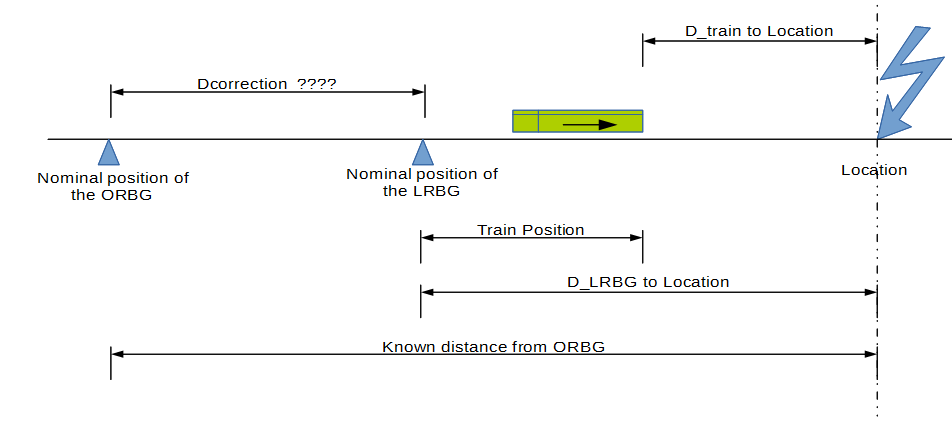
\includegraphics[scale=0.6]{../images/DataStructure_ReferenceSystem_CorrectionDistance.png}
\caption{Calculation of the distance from the train to an a track-side element (“Location”)}\label{fig:ReferenceSystemForCorrection}
\end{figure}
\FIXME{for this principle a justification and design decision is needed}

Therefore for each BG already passed, in reference to which the location of any track-side element is given a minimum and maximum correction distance shall be stored in order to be able to calculate the minimum and maximum distance between the train front end and the track-side element: 

Distance between train and location =
Distance from ORBG – Train Position (I.r.t. LRBG)  -  the stored correction distance (all including tolerances).


As the Location of a track-side element can also be given in reference to a BG in advance of the train (infill information), the same correction distance shall be available for announced BG's. This is only with one difference. For announced BG the exact linking distance is available (if not the infill information can and must not be taken into account). The correction distance exact (no minimum and maximum), and equal to the linking distance.

This leads to the need for two data structures, one storing the correction distances for already passed BG's, and one storing the announced (linking) distance from the nominal position of the LRBG to the announced BG's. The latter structure also contains the data needed for checking the linking consistency, i.e. the expectation window. A graphical representation of the data structure is given below: 

\begin{figure}[ht]
\centering
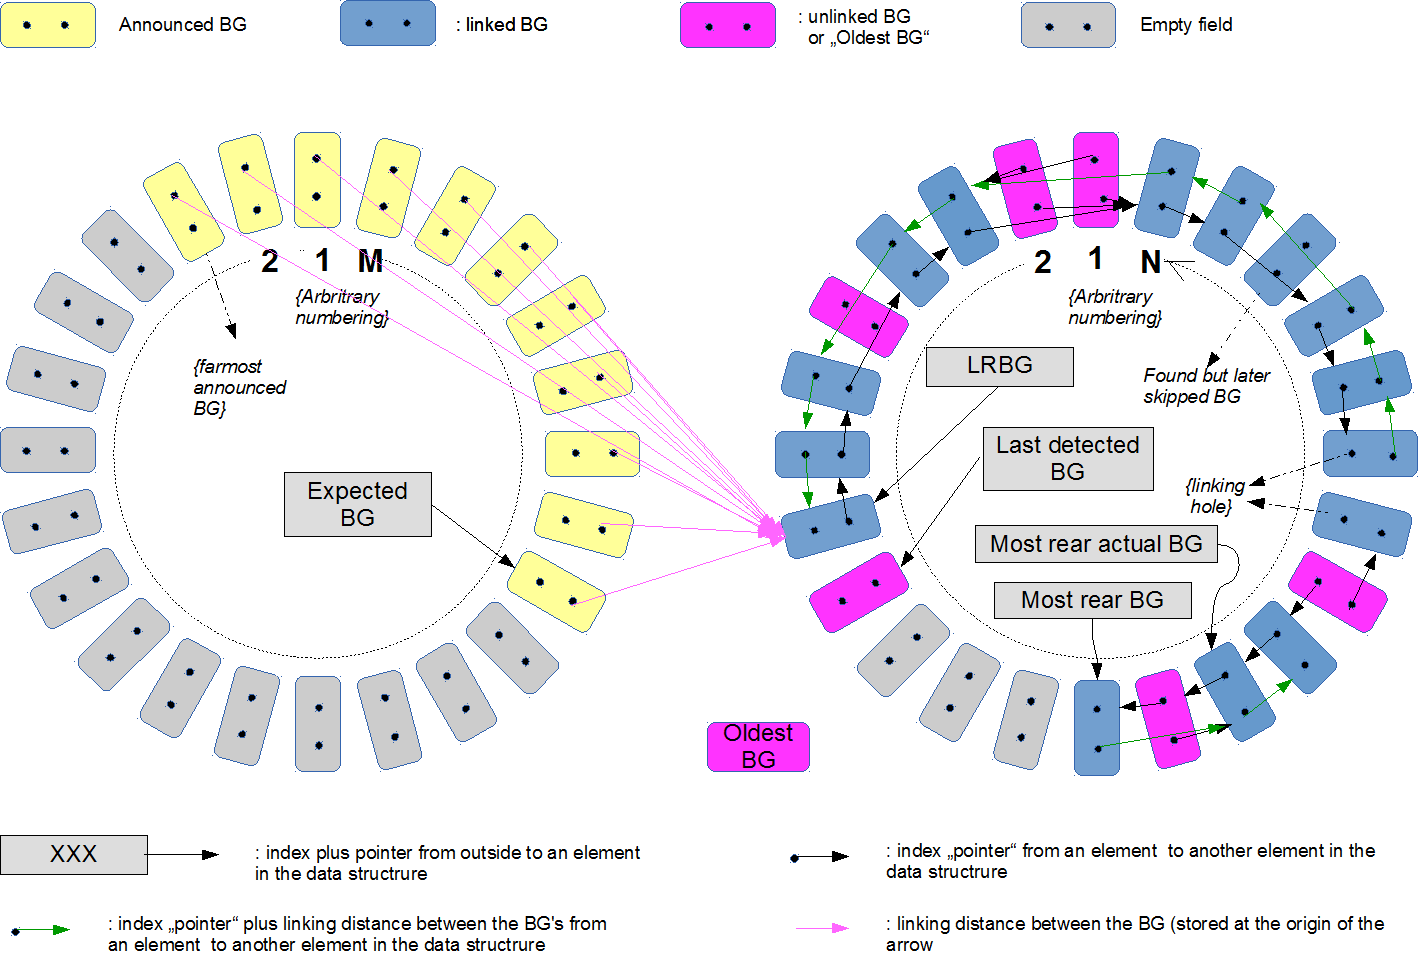
\includegraphics[scale=0.4]{../images/DataStructure_Linking.png}
\caption{Data structures for announced,  detected linked and detected unlinked BG's}\label{fig:DataStructureLinking}
\end{figure}

\FIXME{for this principle a justification and design decision is needed}



\begin{enumerate}
\item LRBG: “last relevant BG” = the last detected linked BG
\item Last detected BG: can be different from the LRBG if the last detected BG is marked as “unlinked”
\item Most rear actual BG:  most rear BG to which one or more “Locations” refer as being their ORBG ( original reference BG). All BG's more in rear may be deleted from the list.
\item Most rear BG: the most rear BG whose information is still stored in the “list of detected BG's”
\item “Oldest BG”: BG to which all “Locations” with an ORBG in rear of the “most rear BG” refer. This is used if the “List of detected BG's” is full. Between the “oldest BG” and the “most rear BG” no linking distance is available. Therefore the accuracy for the concerned locations will decrease.
linking hole: Number of linked BG's for which no linking information is available (see figure xx).
skipped BG: Linked BG which was detected when no BG's were announced, but which is not included in linking information received after wards (see figure xx)
“pointer”:  index of the element in the data structure where is referred to.
\end{enumerate}

\subsubsection{Direct orders}
Direct orders can be given for several actions, e.g. command the service or emergency brake, “stop if in staff responsible” etc. Direct orders which have immediate effect at the first evaluation like direct level and mode transitions (have immediate effect in the functional block “filtering” because they shall be taken into account at filtering further information in the message) can be rejected. 
Direct orders shall be stored in the internal data structure to allow the correct execution of the order by the concerning functional block. For each possible order a field shall be reserved, i.e. an array with a field for every possible order shall be build.

This data structure is needed to avoid getting event driven software, as the orders are stored and read by the a functional block which is commanded cyclically.
Direct orders to be stored (as a flag or variable):
\begin{itemize}
\item command service brake
\item “stop in staff responsible”
\item SR authorisation
\item Exit of trip mode
\item Inhibition of revoking TRS's
\end{itemize}
\FIXME{List needs to be completed by all orders including a special value ``now'' according to SUBSET-026-7}

\FIXME{ To what extent shall mode changes following from input data be taken into account before filtering?}

Intermediate analysis results (linking error, nb of missed BG's, intervention curve passed,......)
Just like direct orders, some analysis results shall lead to a certain specified action. For example, having a consistency error shall lead to the linking reaction (given from track-side or the default value which is command service brake). Just like direct orders those intermediate results are stored as an order for other functional blocks, in stead of immediately (event driven) calling the specific function.
Intermediate results to be stored (as a flag or variable):
\begin{itemize}
\item From BCM: EB intervention, SB intervention, acoustical warning, Vsoll, Vwarning,...
\item From linking consistency checking: type of linking reaction, number of missed BG's
\item From message consistency checking: type of linking reaction
…...
\FIXME{needs to be completed}
\end{itemize}

\subsubsection{BG lists for shunting and staff responsible}
Together with the order to go to shunting or to staff responsible a list of BG's which may be passed can be given. Both sets need to be storable in parallel.
The data structure shall consist of an array storing the identities of the BG's which may be passed. As the passing order is not always predictable it doesn't make sense to reorder them. BG's may thus be stored in the same order as they were received.


\subsubsection{Data describing the train } \label{sss:datadescribingthetrain}
To allow the usage of the system on all different train types, data describing the specific train shall be stored. The source of the data can be the TIU, the data entry unit or default values. Data to be stored includes:
\begin{itemize}
\item Train category(-ies)
\item Train length
\item Traction / brake parameters
\item Maximum train speed
\item Loading gauge
\item Axle load category
\item Traction system(s) accepted by the engine
\item Train fitted with airtight system
\item List of National Systems available on-board
\item Number of axles
\end{itemize}
Each parameter shall have a flag to indicate if this parameter can be edited by the driver.
Each parameter shall have a flag to indicate if this parameter can be displayed on demand by the driver.


\subsubsection{Data describing national ruling}
Maximum speeds, braking curve margins, roll away distance, timing for certain conditions, procedural information etc. may differ from country to country.
Therefore a list of national values is defined according to SUBSET-026-A3.2. These national values shall be stored on board, to be available for all functional blocks. 

For those national values, defaults can be defined for the case no national values have been received from track-side. A similar structure shall be provided to remember those default values.


\subsubsection{Track Data}
The version of the track-side ETCS system and the priority of levels supported from track-side shall be available for the functional blocks. Data structures to store this information in the same format as it is received from track-side shall be provided.


\subsubsection{Driver Data}
Driver data is used when displaying data to the driver (language) and for juridical recording (driver ID). A data structure shall be defined to store all possibly available driver data, see also chapter \ref{sss:datadescribingthetrain}


\subsubsection{Procedure status information}
In the SRS (especially SUBSET-026 chapter 5) a number of procedures between track-side, train and driver are described, e.g.
\begin{itemize}
\item data-entry
\item reporting train position
\item SoM, EoM
\item override
\item Train data management....
\item text message acknowledgements
\item establishing and ending a connection to the RBC
\item RBC-RBC hand over
\item transition to shunting
\item transition to staff responsible
\item …...
\item \FIXME{complete procedure}
\end{itemize}

For each of these procedures the status shall be remembered, in some cases including the time since specific events.
Therefore for each procedure a global data structure shall be designed to remember the status of each procedure.


\subsubsection{Parameters for procedures}
As the requirements concerning procedures may differ, parameters are defined to tune the procedures. (timing requirements, etc.). Data structures to store this information in the same format as it is received from track-side shall be provided.


\subsubsection{System mode and level}
The system mode and level shall be available to all functional blocks at any time. Therefore variables to store the current state and level shall be defined.


\subsubsection{System status}
Data structures are necessary to store the current status of the subsystems (Radio, BTM, LTM, STM, JRU, odometer, TIU, brakes). 


\subsubsection{Data structures to store messages to be sent to the RBC}
The information needed which as to be sent to the RBC is provided by “train supervision”, “mode/level management”, diverse procedures etc. 
To sent them to the RBC the information has to be build in a specific format (specified in ss026, chapter 7 and 8). This structure has to be synchronised with the API specification


\subsubsection{Data structures to sent to subsystems (DMI, TIU/BIU, JRU, STM)}
Information to be sent to the DMI and TIU/BIU shall be build in data structures as described in the API specification.
The JRU and STM are out of scope for the current iteration.



 
\section{Management of location based data}
A lot of information given from ETCS track side to on-board is “Location based”, i.e. the information is valid for a certain location given as a distance from a reference BG. The current function will manage the elaboration of packets containing “Location based data” into the (already available) sorted internal data structures which shall enable efficient further elaboration of the data (e.g. braking curve monitoring, constituting the planning area, etc.).

\textbf{Description:}
Elaboration of the packets containing “Location based data” into the (already available) sorted internal data structures.

\textbf{Inputs:} 
\begin{itemize}
\item Packets containing “Location based data” (see below)
\end{itemize}

\textbf{Affected data in the “data stored on-board”: 	}
\begin{itemize}
\item Internal data structures storing “internal data structures” 
\item Status of received packets (change to “elaborated”, thus may be forgotten) 
\end{itemize}
\textbf{Outputs:}  -

“Location based” data is categorized for the purpose of defining data structures:
\begin{itemize}
\item \textbf{movement authority (MA) list of sections}, message 37, packet 12 (level 1), message 3, packet 15 (level 2), 16 (repositioning, i.e. extending the current section), message 33 (??), packet 70 (route suitability), message 9 (request to shorten MA),    minimum number of elements to be stored: 6
\item \textbf{list of announced BG's linking information:} packet 5  minimum number of elements to be stored: 30
\item \textbf{adhesion factor:} packet 71;  only one element
\item the \textbf{“gradient profile”} (in: pkt 21)  minimum number of elements to be stored: 50
\item \textbf{Speed profiles:}  packet 27 (SSP)  {the worst case can be determined at reception} 
Packet 13	minimum number of elements to be stored: 50
\item \textbf{Speed restrictions} and non-continuous speed profiles: packet 51 (axle load profile), packet 52 (permitted braking distance), packets 65/66 (TSR), packet 88 (level crossing, incl. stop condition to be reset at standstill).  
minimum number of elements to be stored: TSR: 30, axle load: 30, permitted braking distance:  5 , level crossing: 10. 
Reversing area's: packets 138, 139	minimum number of elements to be stored: 1
Mode dependent speeds: message 2  and packet 80  minimum number of elements to be stored: 6
\item \textbf{Level transitions:} packet 41  minimum number of elements to be stored:  (see ss26, 5.10.1.6): 1
\item \textbf{RBC Transitions:} packet 131
\item \textbf{Radio infill area entry or exit:} packet 133
Loop announcement: packet 134
\item \textbf{Conditional emergency stop:} message 15
\item \textbf{DMI information:} packets 72,76 (text messages), packet 79 (geographical position information), message 34 (track ahead free request)  minimum number of elements to be stored: fixed text: 5, free text: 5, geographical position: 
\item \textbf{Track conditions} (to be passed to the TIU and displayed at the DMI): packet 39 (traction system), packet 40 (current limitation),  packet 68 (diverse track conditions), packet 69 (platform conditions). Pkt 139  minimum number of elements to be stored: 20, + 1 for change power supply + 1 for platform conditions, + 1 for current limitation
\item \textbf{Route suitability:} minimum number of elements to be stored: 3
\item \textbf{Big Metal Mass:} Technical information (to be used for BG-filtering): packet 67 (ignore BG integrity)  minimum number of elements to be stored: 5
\item \textbf{Virtual balise covers:}  minimum number of elements to be stored: 10
\item \textbf{list of position report locations.} In: pkt. 58  minimum number of elements to be stored: 15
\end{itemize}

All above information contains “Locations”. These “Locations” can all be managed in the same manner. A location is defined using the following data structure:

For each location the “original reference” (ORBG) and the distance from this ORBG are remembered. 
In the data structure for passed BG's a correction distance is stored such that:

\begin{figure}[hbtp]
\centering
\includegraphics[angle=0, scale=0.9] {images/ORBG.png}
\caption{SRS architecture}
\end{figure}


$d_{ between~train~and~location} =
d_{from~ORBG} - P_{Train~to~ LRBG}  -  d_{correction~stored}$

\FIXME{formula needs to be documented with a picture or refined description of the variables}

where
\begin{description}
   \item[$d$] - represents a distance
   \item[$P$] - represents the train position
\end{description}
$the stored correction distance (all including tolerances)$.

A location is thus always stored as a distance from the nominal location of the ORBG (thus not having tolerances). Location based data is given from track-side as a chain of incremental distances. This shall be converted during the elaboration and storage.

Typically location based data has to be available in the order it is passed. This requires ordering and reordering if an element The following situations have to be taken into account:
\begin{itemize}
\item some types of location based data are not sent in the order they are passed, i.e. an element can be received which has to be included halfway the list.
\item some types of location based data can be withdrawn from the list.
\item Some types of location based data can be updated
\item Information stored for a location can change, e.g. if the axle load changes, then the speed restrictions stored for this item shall be changed.
\item Shifting of data shall be avoided.
\end{itemize}

\begin{figure}[hbtp]
\centering
\includegraphics[angle=0, scale=0.6] {images/indexing_of_ringbuffer.png}
\caption{Indexing of internal data structure}
\end{figure}


General data structure for location based data of a specific type: “LOCATION BASED DATA STRUCTURE”
\begin{description}
\item[closest:] The element related to the location which is the closest to the train front end
\item[furthest:] The element related to the location which is the closest to the train front end
\item[first free:] The element where the next received “location based data element of the specific type
\end{description}

Each element shall contain the index of the element where the preceding location is stored,  the index of the element where the next further location is stored, the location (see type description above) and fields for information depending of the type of location based data.


\begin{figure}[hbtp]
\centering
\includegraphics[angle=0, scale=0.9] {images/location_based_datastructure.png}
\caption{Location based data structure}
\end{figure}

Generic structure for an element in a data structure for location based data


General functions to be performed on a “LOCATION BASED DATA STRUCTURE” when new information is received are:
\begin{itemize}
\item Replace all data from a certain location onwards with the new received information.
\item Insert one element in the structure at the right location, i.e. between the last preceding and the first next location of the same type.
\item Delete one element of the structure, i.e. restore the order and free the memory where the information was stored.
\item Update the information for a specific (already stored) element containing location based data, e.g. update the speed of “axle load dependent speed restrictions” in case the axle load changes.
\end{itemize}

\textbf{ORDER IN WHICH PACKETS CONTAINING LOCATION BASED DATA SHALL BE ELABORATED}

There are a few requirements determining the order in which different types of data shall be analyzed:
\begin{itemize}
\item MA's may only be accepted if a static speed profile and gradient information is available. Therefore the latter ones shall be elaborated before the MA information is elaborated.
\item xxxx
\end{itemize}

Scope of the function
The current function includes all elaboration of packets containing location based data into the internal data structure for location based data, further elaboration is not included.
MRSP and the list of targets for braking curve monitoring are also location based, but they are a further elaboration of the received data. The building of the MRSP and list of braking curve targets is therefore not handled in the current function but in “Build MRSP + list of targets at the LRBG” (see figure~\ref{fig:lbd}).


\begin{figure}[hbtp]
\centering
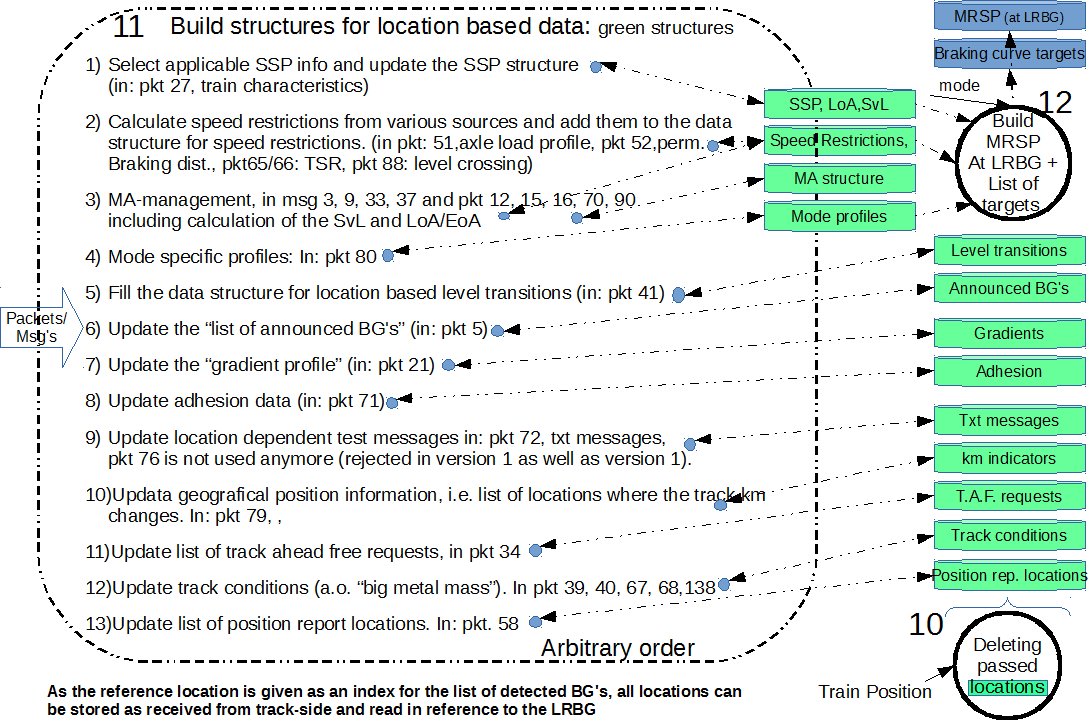
\includegraphics[angle=0, scale=0.55] {images/build_structure_for_location_based_data.png}
\caption{Build Structure of Location Based Data}
\label{fig:lbd}
\end{figure}

 
 \newpage
 \chapter{current partly openETCS Architecture - first iteration}
 Needs to be integrated into the overall architecture .....
  \begin{figure}[hbtp]
\centering
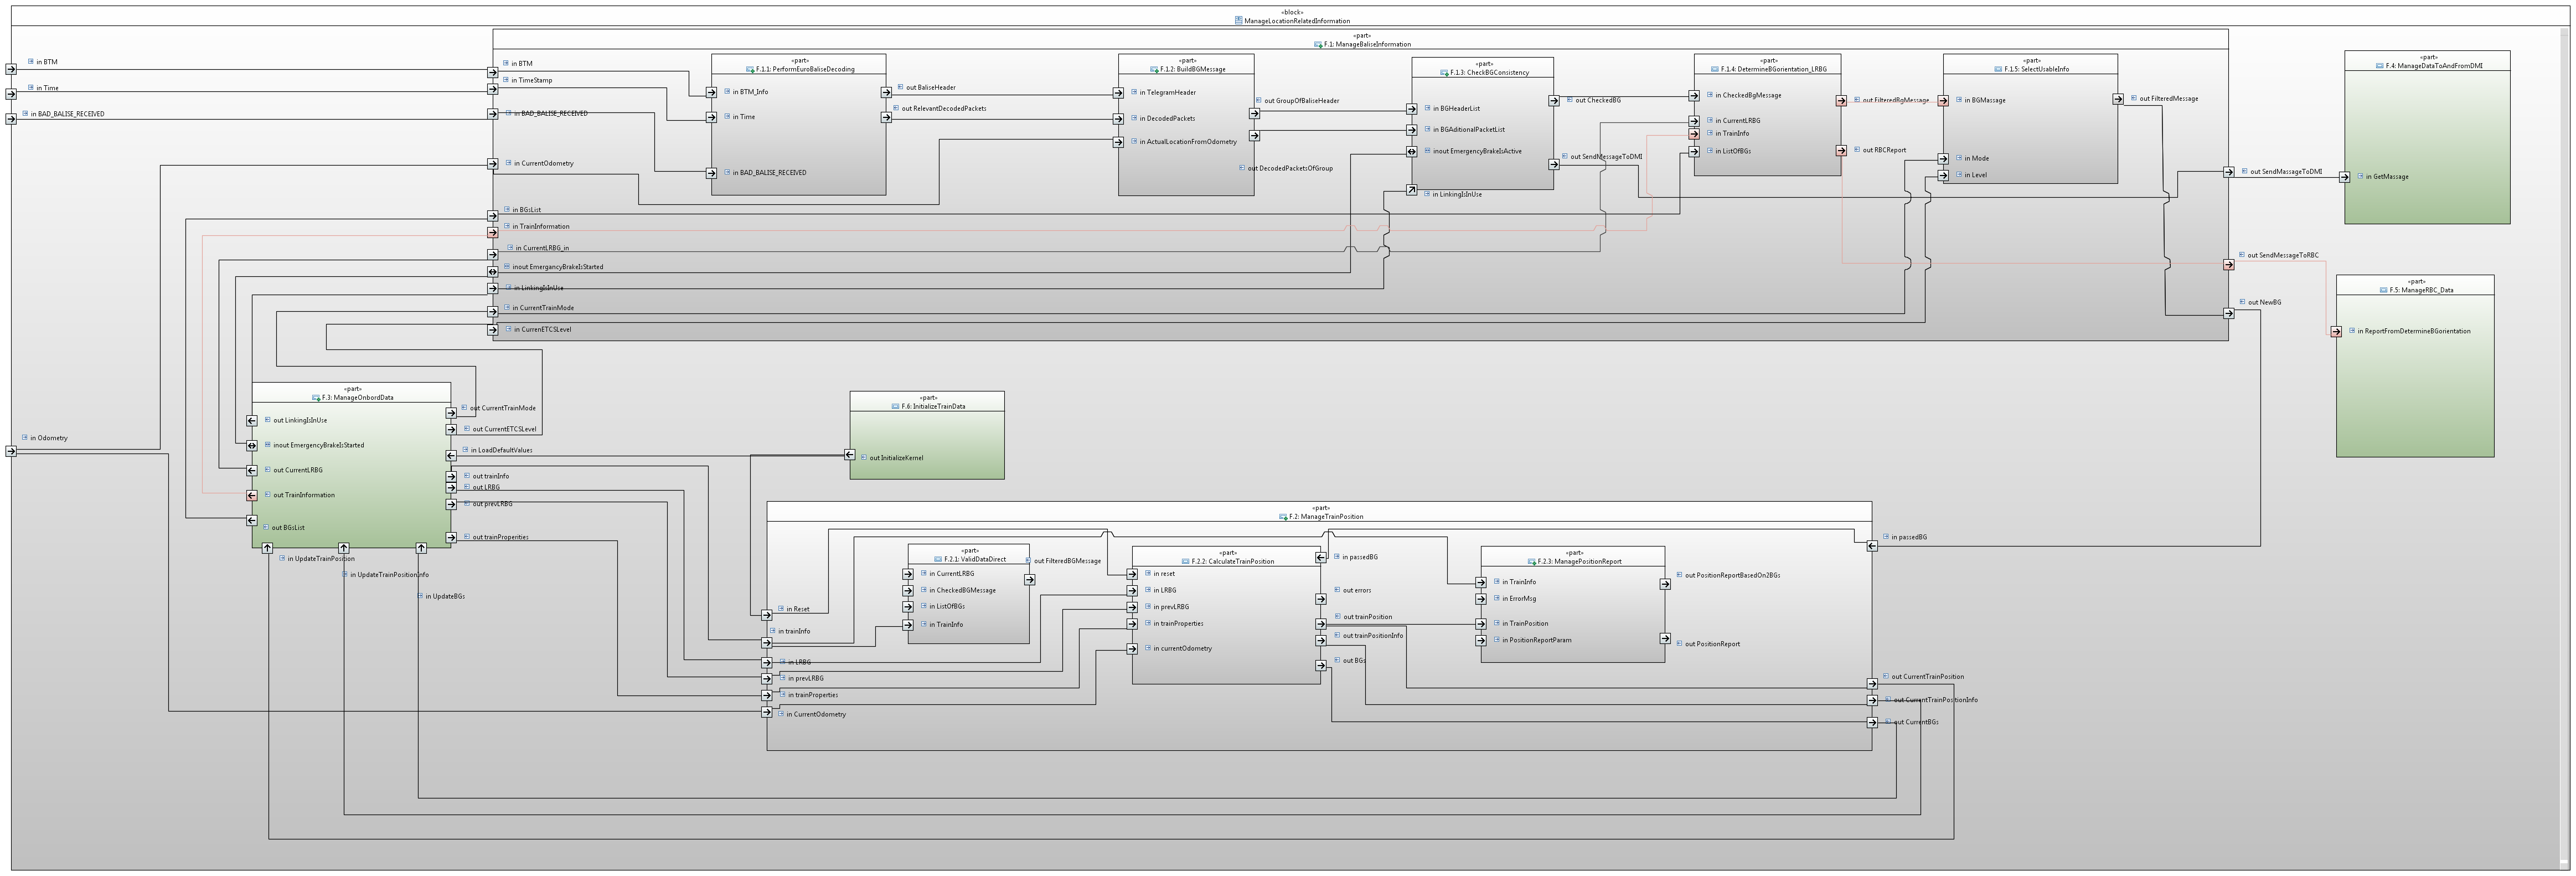
\includegraphics [angle=90, scale=0.2]{images/Current_partly_openETCS_architecture}
\caption{partly openETCS architecture - first iteration}
\end{figure}
 
 \newpage
  \chapter{merge the first iteration architecture with the overall architecture}
 Needs to be integrated into the overall architecture .....
  \begin{figure}[hbtp]
\centering
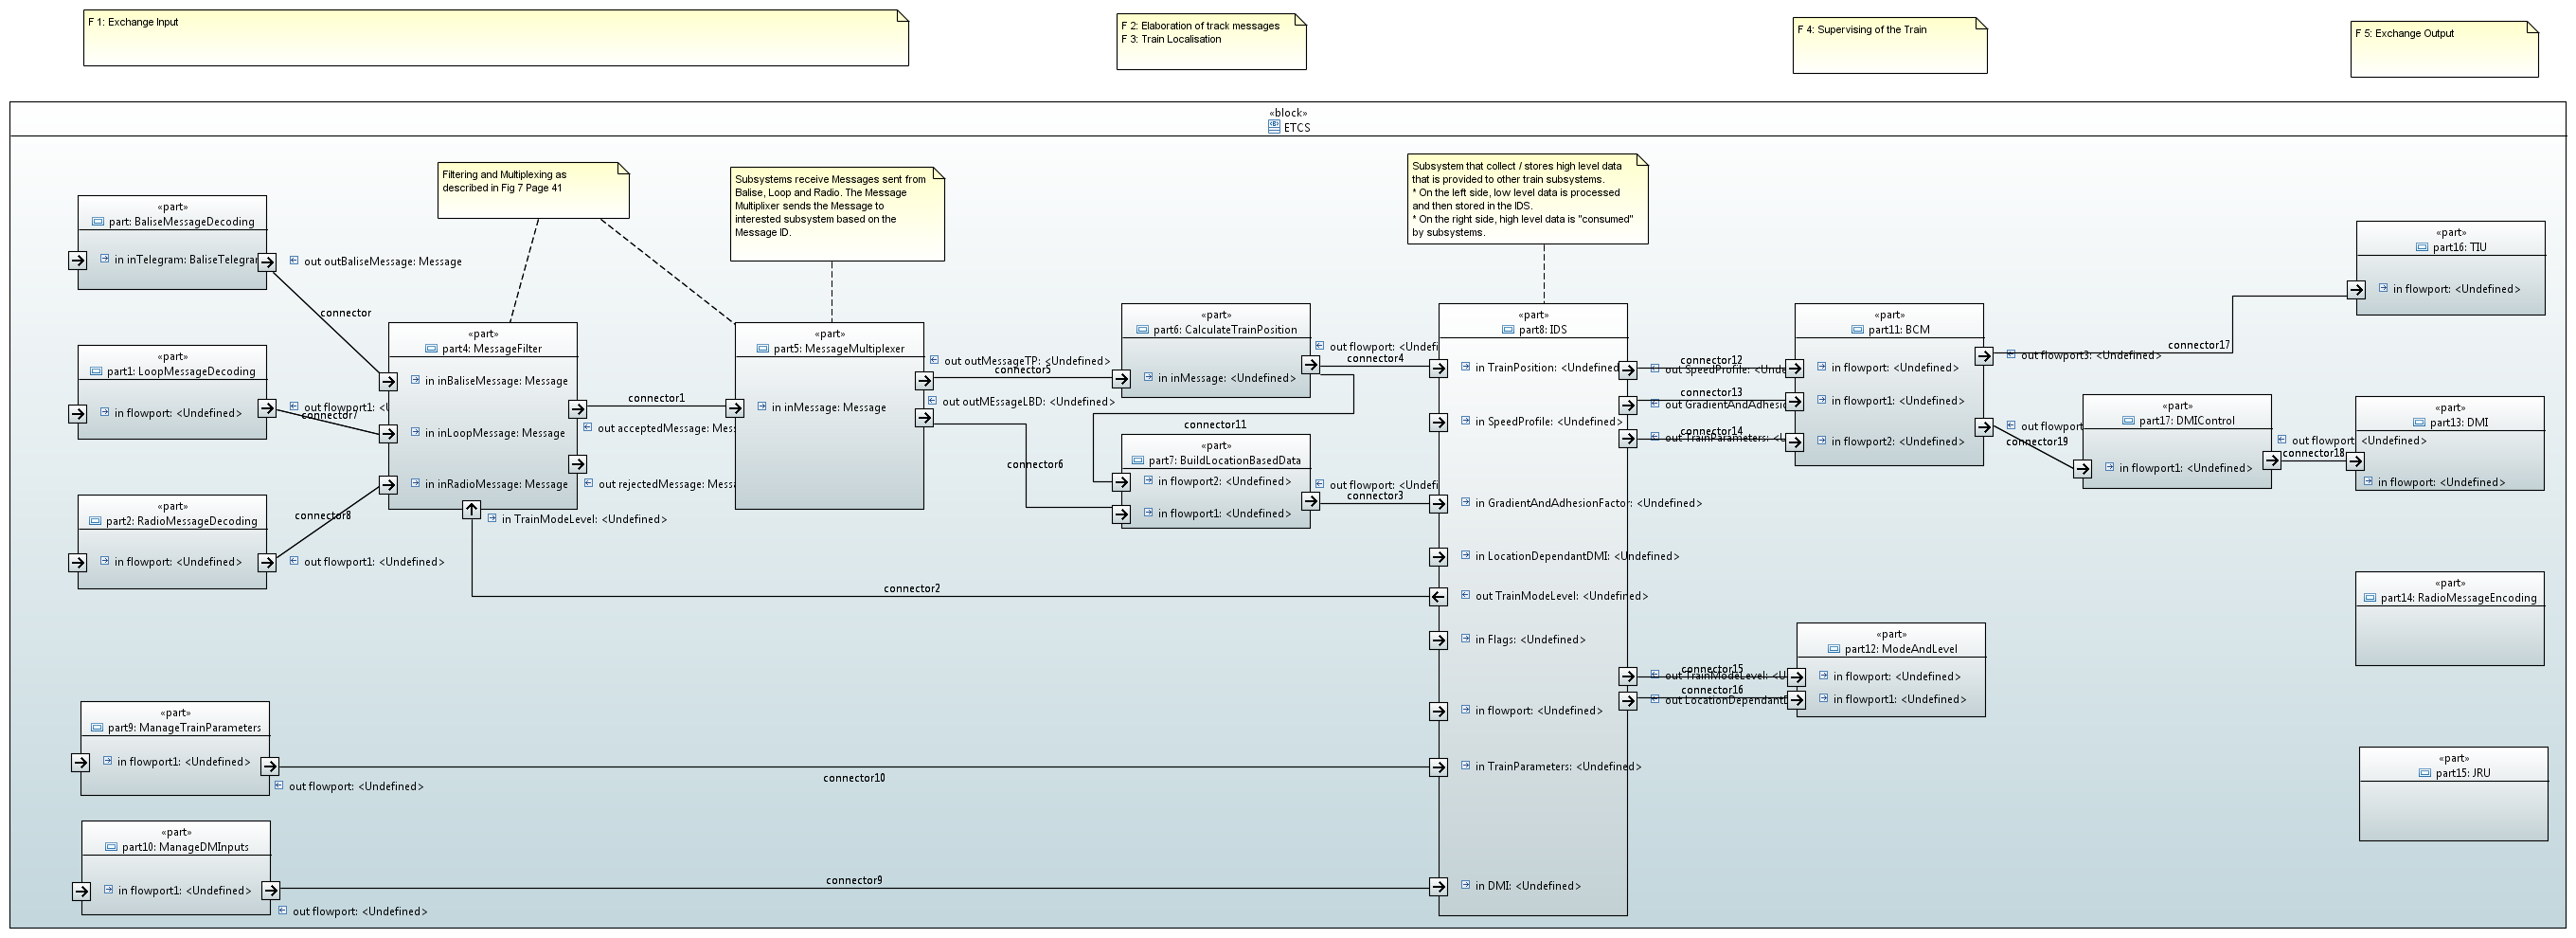
\includegraphics [angle=90, scale=0.3]{images/architecture-db}
\caption{concept to merge}
\end{figure}
 
% Centralizes data structure has been detailed on inside chapter "Functional and data structure architecture ETCS on-board"
% \newpage
% \chapter{centralized data structure approach}
% \begin{figure}[hbtp]
%\centering
%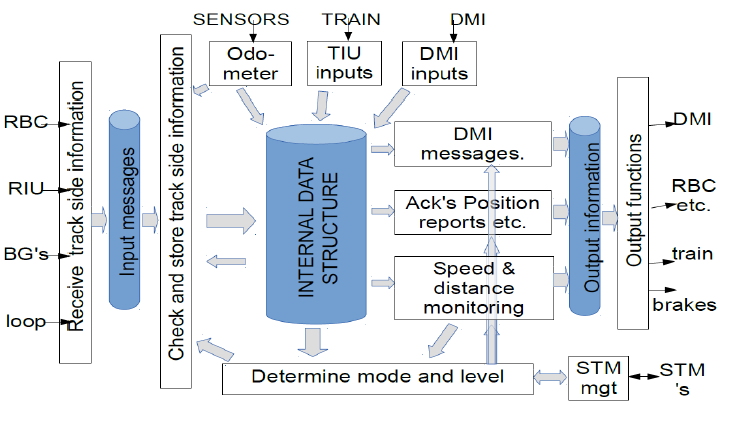
\includegraphics [scale=0.6] {images/CentralizedDataStrukture_2}
%\caption{Centralized data structure approach architecture}
%\end{figure}


% \begin{figure}[hbtp]
%\centering
%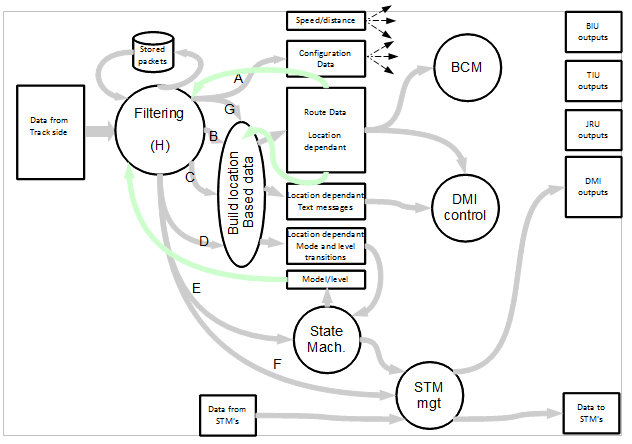
\includegraphics [scale=0.7] {images/CentralizedDataStructure_1}
%\caption{Centralized data structure approach breakdown}
%\end{figure}

\newpage

\chapter{Alstom High Level Approach}
 \begin{figure}[hbtp]
\centering
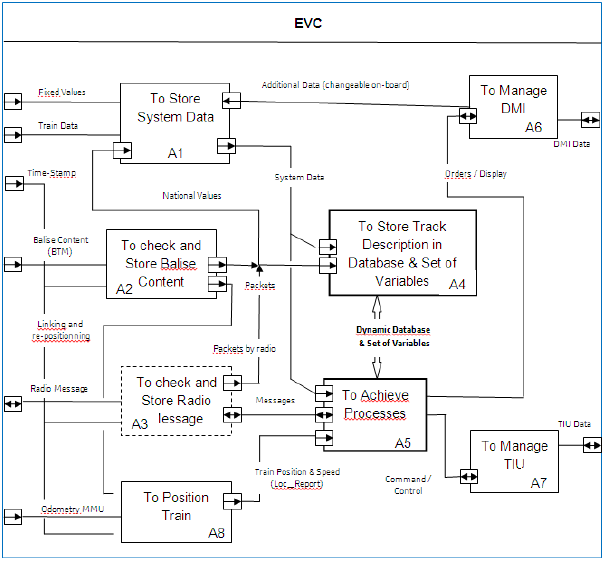
\includegraphics [scale=0.8] {images/Alstom_High_Level_Approach}
\caption{Alstom SRS Architecture Approach}
\end{figure}

\newpage

 
\appendix

\bibliographystyle{unsrt}
\bibliography{architecture}

\newpage
\addcontentsline{toc}{chapter}{Index}
\printindex

%===================================================
%Do NOT change anything below this line

\end{document}
